%%%%%%%%%%%%%%%%%%%%%%%%%%%%%%%%%%%%%%%%%
% Bachelor/Master Thesis 
% LaTeX Template
% Version 2.5 (27/8/17)
%
% This template was downloaded from:
% http://www.LaTeXTemplates.com
%
% Version 2.x major modifications by:
% Vel (vel@latextemplates.com)
%
% This template is based on a template by:
% Steve Gunn (http://users.ecs.soton.ac.uk/srg/softwaretools/document/templates/)
% Sunil Patel (http://www.sunilpatel.co.uk/thesis-template/)
%
% Template license:
% CC BY-NC-SA 3.0 (http://creativecommons.org/licenses/by-nc-sa/3.0/)
%
%%%%%%%%%%%%%%%%%%%%%%%%%%%%%%%%%%%%%%%%%

%----------------------------------------------------------------------------------------
%	PACKAGES AND OTHER DOCUMENT CONFIGURATIONS
%----------------------------------------------------------------------------------------

\documentclass[
11pt, % The default document font size, options: 10pt, 11pt, 12pt
%oneside, % Two side (alternating margins) for binding by default, uncomment to switch to one side
english, % ngerman for German
singlespacing, % Single line spacing, alternatives: onehalfspacing or doublespacing
%draft, % Uncomment to enable draft mode (no pictures, no links, overfull hboxes indicated)
%nolistspacing, % If the document is onehalfspacing or doublespacing, uncomment this to set spacing in lists to single
liststotoc, % Uncomment to add the list of figures/tables/etc to the table of contents
toctotoc, % Uncomment to add the main table of contents to the table of contents
%parskip, % Uncomment to add space between paragraphs
%nohyperref, % Uncomment to not load the hyperref package
headsepline, % Uncomment to get a line under the header
%chapterinoneline, % Uncomment to place the chapter title next to the number on one line
%consistentlayout, % Uncomment to change the layout of the declaration, abstract and acknowledgements pages to match the default layout
% oneside % to avoid doublepage
]{BachelorMasterThesis} % The class file specifying the document structure

\usepackage{booktabs} % required for tables
\usepackage[utf8]{inputenc} % Required for inputting international characters
\usepackage[T1]{fontenc} % Output font encoding for international characters

\usepackage{mathpazo} % Use the Palatino font by default
% \usepackage[backend=bibtex,style=authoryear,natbib=true]{biblatex} % Use the bibtex backend with the authoryear citation style (which resembles APA)

% \addbibresource{main.bib} % The filename of the bibliography

\usepackage[autostyle=true]{csquotes} % Required to generate language-dependent quotes in the bibliography
\usepackage{amsmath}
\usepackage{graphicx}
\usepackage{caption}
\usepackage{subcaption}
% \captionsetup[table]{position=bottom}

%----------------------------------------------------------------------------------------
%	CUSTOM COMMANDS
%----------------------------------------------------------------------------------------

\newcommand{\mat}[1]{\pmb{\mathsf{#1}}}
\DeclareMathOperator{\rank}{rank}
% \newcommand{\pt}[1]{\mathsf{#1}}

%----------------------------------------------------------------------------------------
%	MARGIN SETTINGS
%----------------------------------------------------------------------------------------

\geometry{
	paper=a4paper, % Change to letterpaper for US letter
	inner=2.5cm, % Inner margin
	outer=3.8cm, % Outer margin
	bindingoffset=.5cm, % Binding offset
	top=1.5cm, % Top margin
	bottom=1.5cm, % Bottom margin
	%showframe, % Uncomment to show how the type block is set on the page
}

%----------------------------------------------------------------------------------------
%	THESIS INFORMATION
%----------------------------------------------------------------------------------------

\thesistitle{Multi-camera visual obstacle avoidance for micro aerial vehicles} % Your thesis title, this is used in the title and abstract, print it elsewhere with \ttitle
\supervisor{Ing. Matouš \textsc{Vrba}} % Your supervisor's name, this is used in the title page, print it elsewhere with \supname
\examiner{} % Your examiner's name, this is not currently used anywhere in the template, print it elsewhere with \examname
\degree{Bachelor of Science} % Your degree name, this is used in the title page and abstract, print it elsewhere with \degreename
\author{Mykola \textsc{Morhunenko}} % Your name, this is used in the title page and abstract, print it elsewhere with \authorname
\addresses{} % Your address, this is not currently used anywhere in the template, print it elsewhere with \addressname

\subject{Robotics, Computer Science} % Your subject area, this is not currently used anywhere in the template, print it elsewhere with \subjectname
\keywords{"micro aerial vehicle, obstacle avoidance, computer vision, robotiks"} % Keywords for your thesis, this is not currently used anywhere in the template, print it elsewhere with \keywordnames
\university{\href{https://ucu.edu.ua}{Ukrainian Catholic University}} % Your university's name and URL, this is used in the title page and abstract, print it elsewhere with \univname
\department{\href{https://apps.ucu.edu.ua}{Department of Computer Sciences}} % Your department's name and URL, this is used in the title page and abstract, print it elsewhere with \deptname
\group{\href{https://apps.ucu.edu.ua/computer-science/}{Faculty of Applied Sciences}} % Your research group's name and URL, this is used in the title page, print it elsewhere with \groupname
\faculty{\href{https://apps.ucu.edu.ua}{Faculty of Applied Sciences}} % Your faculty's name and URL, this is used in the title page and abstract, print it elsewhere with \facname

\AtBeginDocument{
\hypersetup{pdftitle=\ttitle} % Set the PDF's title to your title
\hypersetup{pdfauthor=\authorname} % Set the PDF's author to your name
\hypersetup{pdfkeywords=\keywordnames} % Set the PDF's keywords to your keywords
}

\begin{document}

\frontmatter % Use roman page numbering style (i, ii, iii, iv...) for the pre-content pages

\pagestyle{plain} % Default to the plain heading style until the thesis style is called for the body content

%----------------------------------------------------------------------------------------
%	TITLE PAGE
%----------------------------------------------------------------------------------------

\begin{titlepage}
\begin{center}

\vspace*{.06\textheight}
{\scshape\LARGE \univname\par}\vspace{1.5cm} % University name
\textsc{\Large Bachelor Thesis}\\[0.5cm] % Thesis type

\HRule \\[0.4cm] % Horizontal line
{\huge \bfseries \ttitle\par}\vspace{0.4cm} % Thesis title
\HRule \\[1.5cm] % Horizontal line
 
\begin{minipage}[t]{0.4\textwidth}
\begin{flushleft} \large
\emph{Author:}\\
\authorname % Author name - remove the \href bracket to remove the link
\end{flushleft}
\end{minipage}
\begin{minipage}[t]{0.4\textwidth}
\begin{flushright} \large
\emph{Supervisor:} \\
\href{http://mrs.felk.cvut.cz/members/phdstudents/matous-vrba}{\supname} % Supervisor name - remove the \href bracket to remove the link  
\end{flushright}
\end{minipage}\\[3cm]
 
\vfill

\large \textit{A thesis submitted in fulfillment of the requirements\\ for the degree of \degreename}\\[0.3cm] % University requirement text
\textit{in the}\\[0.4cm]
\groupname\\\deptname\\[2cm] % Research group name and department name
 
\vfill

\includegraphics[height=5cm]{UCU-Apps.png} % University/department logo - uncomment to place it

\vfill
{\large \vspace{-0.5cm} Lviv 2022}\\[4cm] % Date
 
\vfill
\end{center}
\end{titlepage}

%----------------------------------------------------------------------------------------
%	DECLARATION PAGE
%----------------------------------------------------------------------------------------

\begin{declaration}
\addchaptertocentry{\authorshipname} % Add the declaration to the table of contents
\noindent I, \authorname, declare that this thesis titled \enquote{\ttitle} and the work presented in it are my own. I confirm that:

\begin{itemize} 
\item This work was done wholly or mainly while in candidature for a research degree at this University.
\item Where any part of this thesis has previously been submitted for a degree or any other qualification at this University or any other institution, this has been clearly stated.
\item Where I have consulted the published work of others, this is always clearly attributed.
\item Where I have quoted from the work of others, the source is always given. With the exception of such quotations, this thesis is entirely my own work.
\item I have acknowledged all main sources of help.
\item Where the thesis is based on work done by myself jointly with others, I have made clear exactly what was done by others and what I have contributed myself.\\
\end{itemize}
 
\noindent Signed:\\
\rule[0.5em]{25em}{0.5pt} % This prints a line for the signature
 
\noindent Date:\\
\rule[0.5em]{25em}{0.5pt} % This prints a line to write the date
\end{declaration}

\cleardoublepage

%----------------------------------------------------------------------------------------
%	QUOTATION PAGE
%----------------------------------------------------------------------------------------

\vspace*{0.2\textheight}

\noindent\enquote{\itshape Science, my lad, is made up of mistakes, but they are mistakes which it is useful to make, because they lead little by little to the truth.}\bigbreak

\hfill Jules Verne

%----------------------------------------------------------------------------------------
%	ABSTRACT PAGE
%----------------------------------------------------------------------------------------

\begin{abstract}
\addchaptertocentry{\abstractname} % Add the abstract to the table of contents

The 21st century is a time of innovation and exploration in the fields of applied science such as physics, medicine, biology, programming and robotics, as well as their intersections and fusions.
One of the research topics, that have recently gained much popularity, are Micro unmanned Aerial Vehicles (MAVs).
MAVs became smaller, cheaper and more readily available.
The rising popularity and utility of MAVs highlights some of their problems.
One of these problems is their reliance on the Global Navigation Satellite System (GNSS), but due to GNSS inaccuracy in closed environments the MAV needs to have an obstacle avoidance system that is compact and reliable.

In this thesis, developing a compact and reliable visual multi-camera obstacle avoidance system for MAVs is developmed.
Calibration of a non-planar stereo camera setup and extraction of obstacle positions in an unknown environment from pairs of 2D images are tackled in this work.

The proposed solution is designed to run onboard an MAV with a limited computational power considering size, weight and payload limitations.
Performance of a prototype of the designed solution of the designed solution was measured in laboratory experiments.
The result proved that the system is ready for on-drone deployment and real-life tests.

\end{abstract}

%----------------------------------------------------------------------------------------
%	ACKNOWLEDGEMENTS
%----------------------------------------------------------------------------------------

\begin{acknowledgements}
\addchaptertocentry{\acknowledgementname} % Add the acknowledgements to the table of contents

I would like to thank my supervisor Ing. Matouš Vrba and all CTU MRS Group members for the opportunity to have an internship there for the last one and a half year, all of them were kind, they helped me a lot with advice's and shared their experience, CTU FEE for interesting and useful for this thesis courses. 
I want to admire that nothing during my studies would take place without my small family - Ukrainian Catholic University, especially Applied Science Faculty, all teachers and deanery for saving all students from all the worst sides of Ukrainian education system and providing only the best quality education without corruption and plagiarism.
\\

Especially, I want to thank all defenders of my Motherland, The Armed Forces of Ukraine, who protect the whole Europe during the russo-Ukraian war at the cost of their own lives to make it possible for all of us to live in peace and for me to write this thesis.
\\

Finally, I would like to thank my family who supported me during my whole life, my mother Svitlana and my father Roman.
\end{acknowledgements}

%----------------------------------------------------------------------------------------
%	LIST OF CONTENTS/FIGURES/TABLES PAGES
%----------------------------------------------------------------------------------------

\tableofcontents % Prints the main table of contents

\listoffigures % Prints the list of figures

\listoftables % Prints the list of tables

%----------------------------------------------------------------------------------------
%	ABBREVIATIONS
%----------------------------------------------------------------------------------------

\begin{abbreviations}{ll} % Include a list of abbreviations (a table of two columns)
\textbf{UAV} & \textbf{U}nmanned \textbf{A}erial \textbf{V}ehicle\\
\textbf{MAV} & \textbf{M}icro Unmanned \textbf{A}erial \textbf{V}ehicle\\
\textbf{ROS} & \textbf{R}obot \textbf{O}perating \textbf{S}ystem\\
\textbf{DoF} & \textbf{D}egree \textbf{o}f \textbf{F}reedom\\
\textbf{SLAM} & \textbf{S}imultaneous \textbf{L}ocalization \textbf{A}nd \textbf{M}apping \\
\textbf{SfM} & \textbf{S}tructure \textbf{f}rom \textbf{M}otion \\
\textbf{PnP} & \textbf{P}erspective \textbf{n} \textbf{P}oints \\
\textbf{FOV} & \textbf{F}ield \textbf{O}f \textbf{V}iew \\
\textbf{SVD} & \textbf{S}ingular \textbf{V}alue \textbf{D}ecomposition \\
\textbf{MRS} & \textbf{M}ulti \textbf{R}obot \textbf{S}ystems Group\\
\textbf{fps} & \textbf{f}rames \textbf{p}er \textbf{s}econd\\
\textbf{LiDAR} & \textbf{L}ight \textbf{D}etection and \textbf{R}anging\\
\textbf{RMS} & \textbf{R}oot \textbf{M}ean \textbf{S}quared\\

\end{abbreviations}

%----------------------------------------------------------------------------------------
%	PHYSICAL CONSTANTS/OTHER DEFINITIONS
%----------------------------------------------------------------------------------------

% \begin{constants}{lr@{${}={}$}l} % The list of physical constants is a three column table

% % The \SI{}{} command is provided by the siunitx package, see its documentation for instructions on how to use it

% Speed of Light & $c_{0}$ & \SI{2.99792458e8}{\meter\per\second} (exact)\\
% %Constant Name & $Symbol$ & $Constant Value$ with units\\

% \end{constants}

%----------------------------------------------------------------------------------------
%	SYMBOLS
%----------------------------------------------------------------------------------------

\begin{symbols}{lll} % Include a list of Symbols (a three column table)

% Symbol & Name & Unit \\

$\vec{t}$ & a column vector that reresents a point or a vector & \\
$\mat{A}$ & a matrix & \\
$\mat{A}^\top$ & transpose of a matrix & \\
$\mat{R}$ & a rotation matrix 3x3, $\det(\mat{R}) = 1, \mat{R}^\top = \mat{R}^{-1}$ & \\
$\mat{I}$ & the identity matrix & \\
$l$ & a line & \\
$f$ & focal length & \\
$\vec{x} \times \vec{y}$ & cross product of $\vec{x}$ and $\vec{y}$ & \\
$[\vec{x}]_\times$ & such matrix that $[\vec{x}]_\times\vec{y} = \vec{x} \times \vec{y} $ & \\
$\lambda$ & any non-zero scalar & \\
$\lVert \vec{a} \rVert$ & the norm of the vector $\vec{a}$ & \\
 & & \\
 & & \\
 & & \\
 & & \\
 & & \\

% \addlinespace % Gap to separate the Roman symbols from the Greek

% $\omega$ & angular frequency & \si{\radian} \\

\end{symbols}

%----------------------------------------------------------------------------------------
%	DEDICATION
%----------------------------------------------------------------------------------------

% \dedicatory{For/Dedicated to/To my\ldots}

%----------------------------------------------------------------------------------------
%	THESIS CONTENT - CHAPTERS
%----------------------------------------------------------------------------------------

\mainmatter % Begin numeric (1,2,3...) page numbering

\pagestyle{thesis} % Return the page headers back to the "thesis" style

% Include the chapters of the thesis as separate files from the Chapters folder
% Uncomment the lines as you write the chapters

\chapter{Introduction}
\label{chapter:intro}

Micro unmanned aerial vehicles (MAVs) recently saw a rise in usage across various fields. Drones are already wide used in cinematography\footnote{\href{https://coptrz.com/drones-in-filmmaking-the-best-drones-for-the-job/\#:~:text=How\%20drones\%20are\%20used\%20in\%20big\%2Dbudget\%20films}{Coptrz, "How drones are used in big-budget films}} and advertising\footnote{\href{https://www.bangkokpost.com/business/2124327/the-future-of-advertising-could-be-drones\#:~:text=However\%2C\%20using\%20drones\%20is\%20a,automobile\%20shows\%20and\%20other\%20campaigns.}{Bangkokpost, "The future of advertising could be drones"}}, In Ukraine they are very helpful in farming (to apply pesticides to fields)\footnote{\href{https://techukraine.org/portfolio/droneua-solution-of-field-cultivation-by-drones-up-to-1-million-hectares-in-ukraine/\#:~:text=Since\%202019\%2C\%20spraying\%20drones\%20began,not\%20depend\%20on\%20soil\%20moisture.}{DroneUA}}. City emergency departments use UAVs  - firefighters can use them to see and evaluate the situation from the sky, localise the source of fire and deal with that\footnote{\href{https://www.dslrpros.com/firefighting-drones.html}{Fire Fighting Drones}}, sometimes it even can have some fire-extinguishing capsules as projectiles\footnote{\href{https://ieeexplore.ieee.org/stamp/stamp.jsp?arnumber=9328798}{Autonomous Firefighting Inside Buildings by an Unmanned Aerial Vehicle}}. They are also quite popular in military industry.

There is no precise definition of MAV; modern MAVs can even be as small as 5 centimetres, but more generally - it is an Unmanned aerial vehicles (UAVs) with some size and weight limitations.

The inspiration for this project was taken from DJI obstacle avoidance technology introduced with the release of the DJI Mavic 3 drone\footnote{\href{https://www.dji.com/cz/mavic-3}{DJI Mavic 3}} on fifth November 2021. Despite the fact that the idea is old, neither DJI nor MRS nor other research groups have a well-developed visual obstacle avoidance system, the best for now can be Skydio obstacle avoidance system \footnotetext{\href
{https://www.skydio.com/skydio-autonomy}{Skydio autonomy}}, so this direction is very perspective for researchers. Many drones available for sale are costly, and even a well-trained pilot is afraid of crashing. At the same time, autonomous drones are more predictable than a human pilot, behave acording to algorithms and can react much faster, but only if they have a well-designed system running on board, so obstacle avoidance for autonomous MAVs will be both more challenging and more critical in future trends.

While obstacle avoidance considers static objects, collision avoidance is related to averting crashing with moving objects like other MAVs, cars or people. It is a complicated task but more relevant to multi-robot systems, because during interactions between robots they should not brake each other.

There are several obstacle avoidance sensors used by various MAVs: stereo vision \cite{arxiv}, depth cameras (as Intel RealSense), monocular vision \cite{Mejias2010}, lidar (2d or 3d) \cite{Ramasamy2016}, sonar (ultrasonic), time of flight sensors, also combinations of them can be used. In \cite{Rambabu2015} the sensor fusion of ultrasonic and infrared sensors is presented.

Each of them has its pros and cons. 3d lidars are extremely expensive but the most efficient for today; 2d lidars are used for small ground vehicles, but not suitable for most tasks for MAVs (because a car can be modelled as a 2 DoF system, while MAV always has 6 DoF), depth cameras are relatively expensive too, ultrasonic and infrared sensors both have distance limits and other minor issues. Overall, stereo vision is the most promising approach for the nearest future.

\section{Related Works}

The goal of this thesis is to implement an obstacle avoidance system, and expand it to collision avoidance system for autonomous MAVs driven by a Robotic operating system (ROS) using the MRS UAV system \footnote{\href{https://github.com/ctu-mrs/mrs_uav_system}{MRS UAV system}}. 

Firstly it is necessary to calibrate a stereo pair, then implement a structure from motion algorithm for each camera and find moving objects using the fact of overlaping sones for each camera.


\section{MRS UAV system}

\clearpage
\chapter{Preliminaries}

\label{chapter:preliminaries}
\section{Homogenous coordinate systems}

Homogenous coordinates are a tool to simplify certain geometrical operations by adding an extra dimension.
For example, the general scaling, rotation and translation is expressed in non-homogenous coordinates as:
% To transform a point $m=(u, v)^\top$ from cartesian coordinates to homogenous, simply append $1$ as the third coordinate: $m=(u, v, 1)^\top$.

\begin{equation}
    \vec{m}_1 = 
    \pmb{\mathsf{S}} \pmb{\mathsf{R}}
    \vec{m}_0
    + \vec{t},
\end{equation}

\begin{equation}
    \pmb{\mathsf{S}} = \begin{bmatrix} s_x & 0 \\ 0 & s_y \end{bmatrix}, \pmb{\mathsf{R}} = \begin{bmatrix} \cos(\theta) & -\sin(\theta) \\ \sin(\theta) & \cos(\theta) \end{bmatrix}, \vec{t} = \begin{bmatrix} t_x \\ t_y \end{bmatrix},
\end{equation}

where $m_0$ is the original point,
$m_1$ is the transformed point,
$\pmb{\mathsf{S}}$ is a scaling matrix,
$\pmb{\mathsf{R}}$ is a rotation matrix and 
$\vec{t}$ is a translation vector.

The same operations can be expressed in homogenous coordinate system using one matrix multiplication as

\begin{equation}
    \begin{bmatrix} \vec{m}_1 \\ 1 \end{bmatrix} = 
    \pmb{\mathsf{S}}_H \pmb{\mathsf{R}}_H \pmb{\mathsf{T}}_H
    \begin{bmatrix} \vec{m}_0 \\ 1 \end{bmatrix},
\end{equation}
\begin{equation}
    \pmb{\mathsf{S}}_H = \begin{bmatrix} s_x & 0 & 1\\ 0 & s_y & 1 \\ 0 & 0 & 1\end{bmatrix}, \pmb{\mathsf{R}}_H = \begin{bmatrix} \cos(\theta) & -\sin(\theta) & 0 \\ \sin(\theta) & \cos(\theta) & 0 \\ 0 & 0 & 1 \end{bmatrix}, \pmb{\mathsf{T}}_H = \begin{bmatrix} 1 & 0 & t_x\\ 0 & 1 & t_y \\ 0 & 0 & 1 \end{bmatrix} ,
\end{equation}
where $\pmb{\mathsf{S}}_H, \pmb{\mathsf{R}}_H$ and $\pmb{\mathsf{T}}_H$ are homogenous transformation matrices.

So in the homogenous coordinate system, all 2D transformations can be combined and expressed as matrix multiplications.

% \subsection{Vanishing point}
% \begin{figure}[h]
%     \centering
%     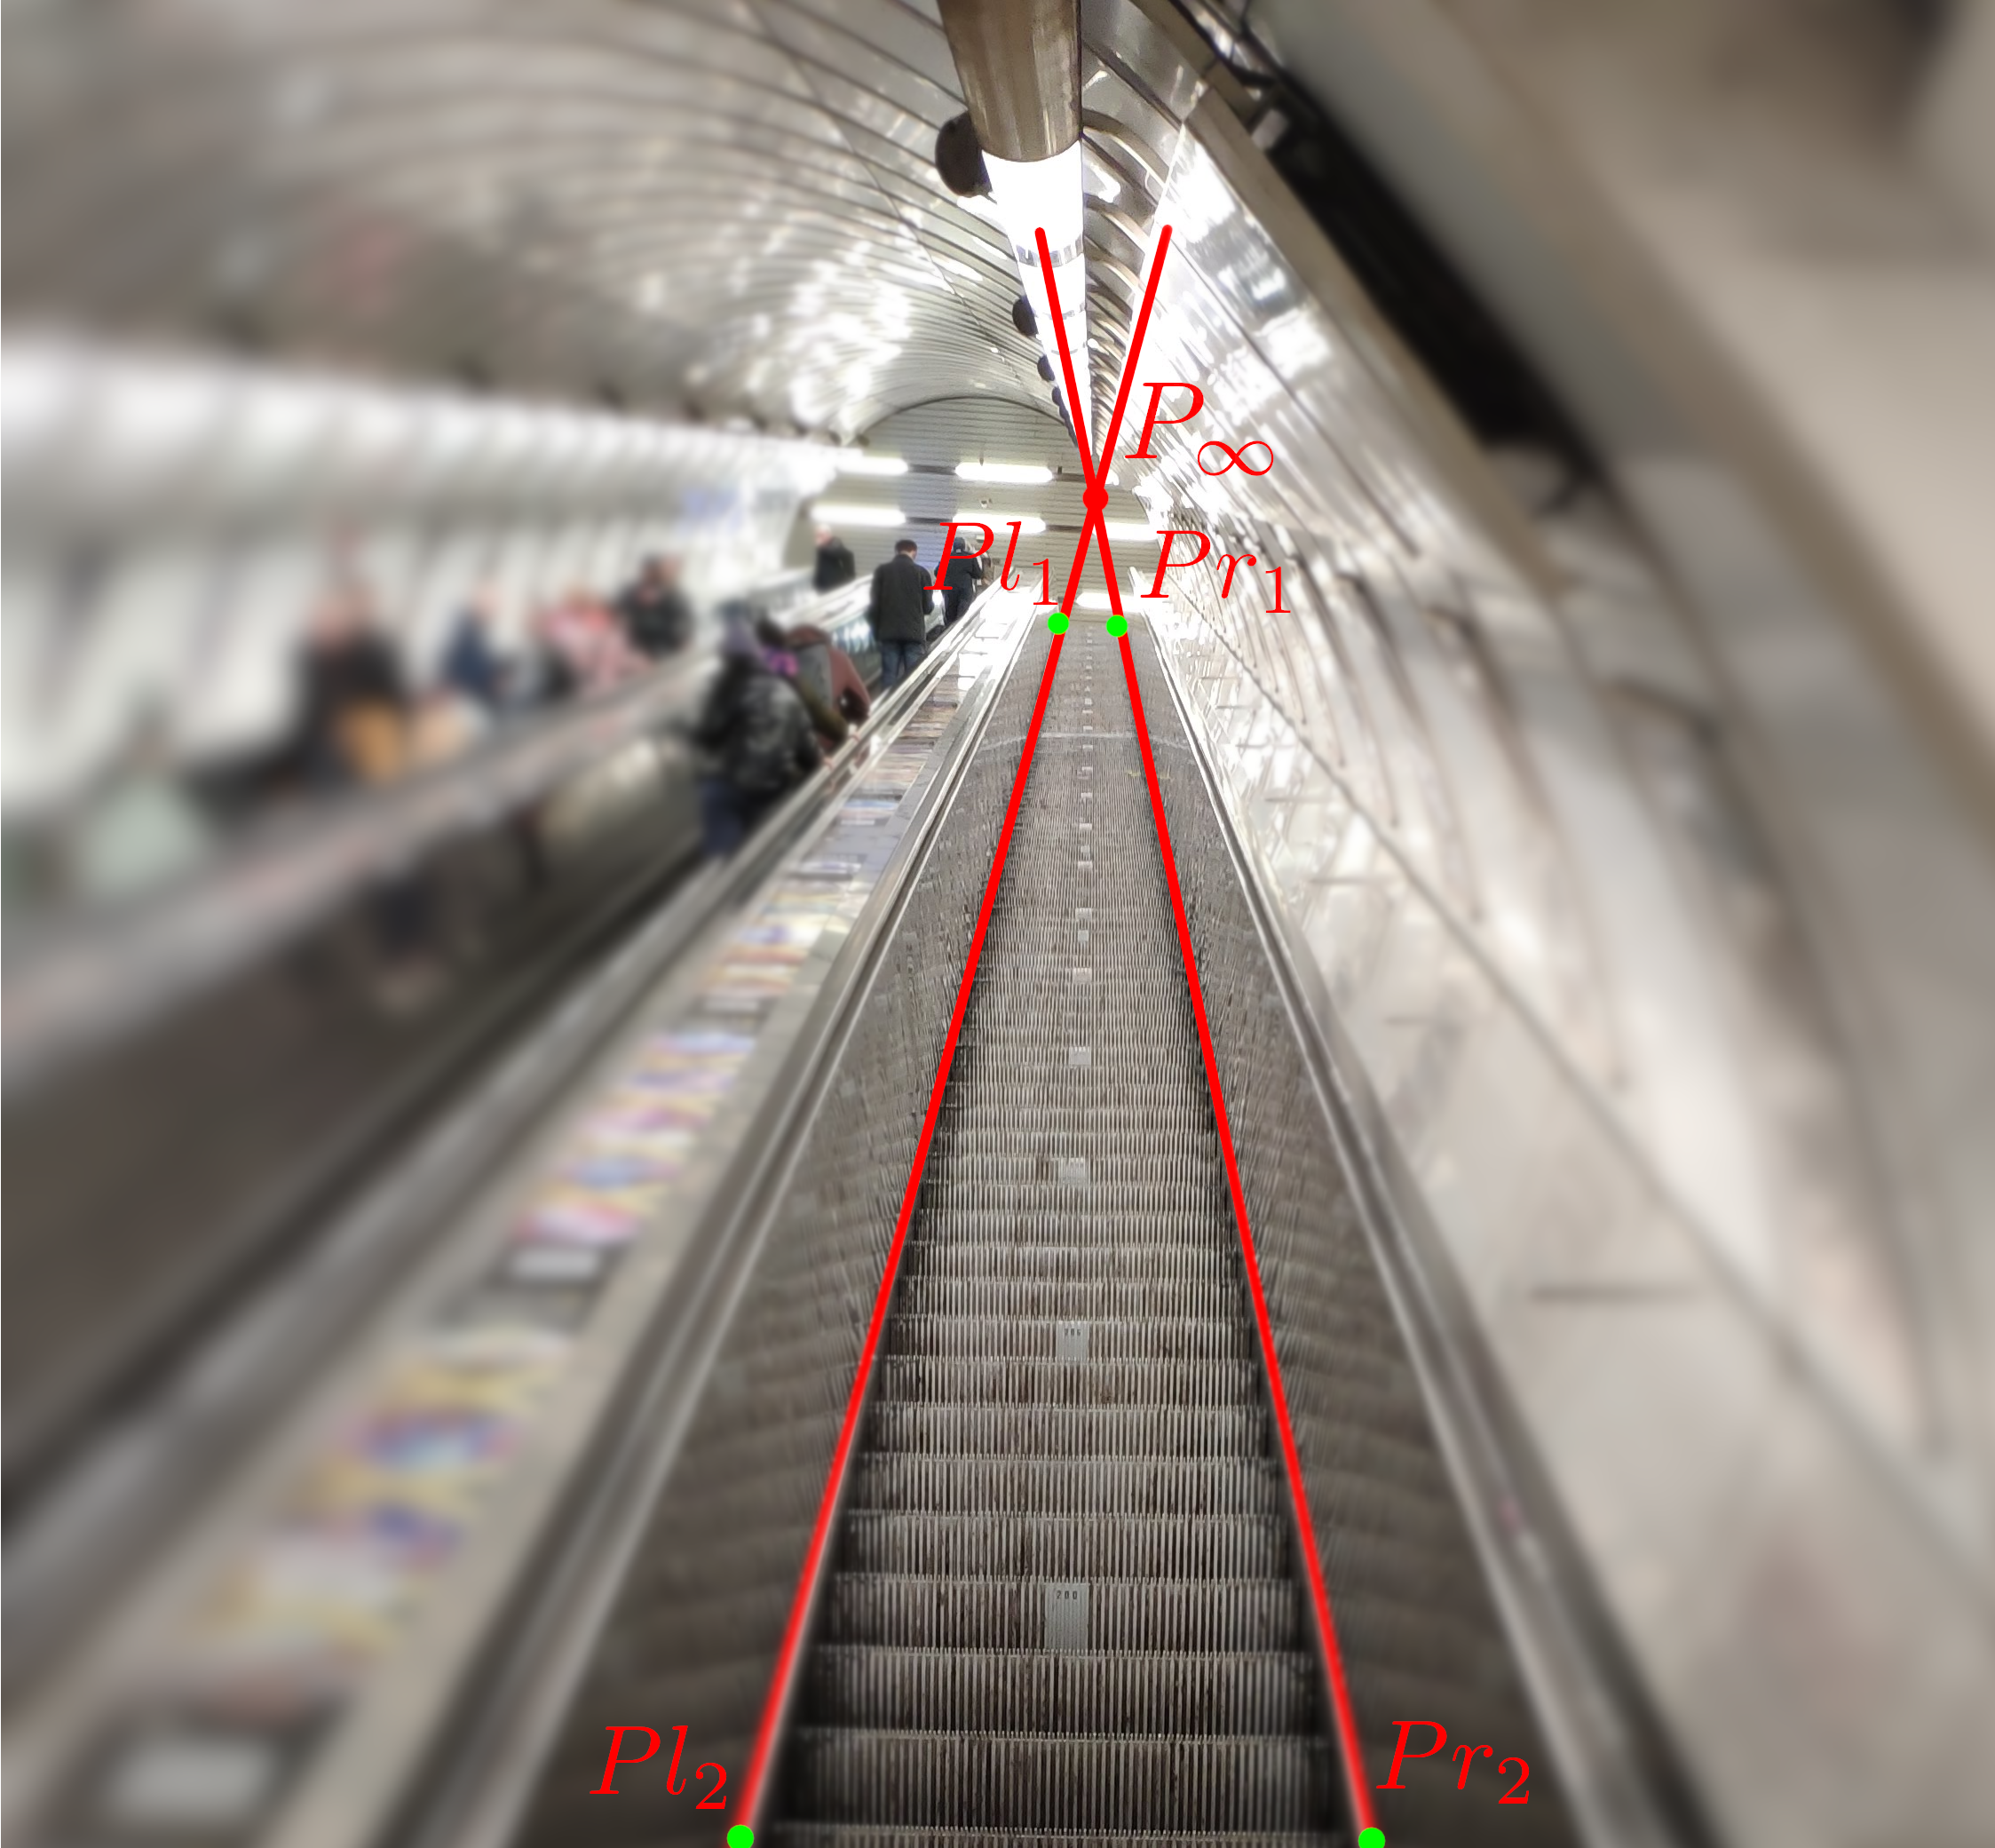
\includegraphics[width=0.75\textwidth]{graphics/parallel_intersection.png}
%     \caption{Parallel lines intersection}
%     \label{fig:intersection_parallel}
% \end{figure}

% \begin{figure}[h]
%     \centering
%     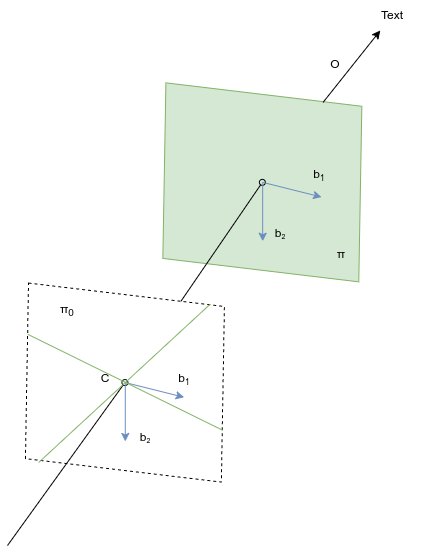
\includegraphics[width=.5\textwidth]{graphics/homogenous.png}
%     \caption{Scheme of homogenous coordinates}
%     \label{fig:homogenous}
% \end{figure}

% In Euclidian geometry, parallel lines are the lines that have no intersection point. 
% In projective geometry, parallel lines intersect at a point $x$ at infinity. 

% In the image \autoref{fig:intersection_parallel} let $l_r$ be a line defined by$Pr_1$ and $Pr_2$, and $l_l$ be a line defined by $Pl_1$ and $Pl_2$. 
% In the 3D world, lines $\vec{l}_l \parallel \vec{l}_r$, but after projection on the image plane $\pi$, lines are interesting at a point $P_\infty$.
% In a general cases, such a point can be computed as a cross product of two parallel lines. 

% Both line and point in a homogenous coordinates are expressed as vectors of three numbers: a homogenous point $\vec{m} = (x, y, z)^\top$ is $\vec{m} = (\frac{x}{z}, \frac{y}{z})^\top$, and a line $\vec{l} = (a, b, c)^\top$, where $a, b, c$ are parameters of a line equation $ax + by + c = 0$. 
% In general case, point at infinity is called an \textit{ideal point} and it is not seen on the image, its coordinates can be expressed as $\vec{m}_{\infty} = (u, v, 0)^\top, \{u, v\} \neq 0$.
% Same about line - such line is called \textit{ideal line} and its coordinates are $\vec{l} = (0, 0, c)^\top, c \neq 0$. In algebraic representation, both ideal point and line are at the plane $\pi_0$ (\autoref{fig:homogenous}, green lines).

% A vanishing point is an image of the point at infinity.
% All world (4D) parallel lines share the same image vanishing point. On a \autoref{fig:intersection_parallel} a $P_{\infty}$ is an image of two parallel lines' intersection point (which is a point at infinity), so it is also a vanishing point.

\section{Pinhole camera model}
A pinhole camera, the canonical perspective camera model - is a model of a simple camera without any optics.
The first example is the camera Obscura - a dark room with a small hole through which the image from outside is projected on the opposite wall. 
This model can be used to express camera geometry with a field of view angles less than $180^{\circ}$.

\subsection{Camera coordinate system}
\begin{figure}[h]
    \centering
    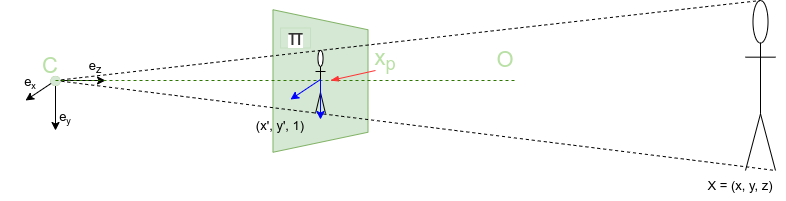
\includegraphics[width=1\textwidth]{graphics/td_scene.png}
    \caption{The scheme of a pinhole camera model}
    \label{fig:td_scene_3d}
\end{figure}

\begin{figure}[h]
    \centering
    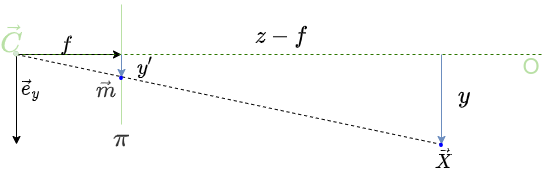
\includegraphics[width=0.9\textwidth]{graphics/td_scene_yz.png}
    \caption{The pinhole camera model, y-z plane}
    \label{fig:td_scene_yz}
\end{figure}

\begin{figure}[h]
  \begin{subfigure}[b]{0.5\textwidth}
    \centering
    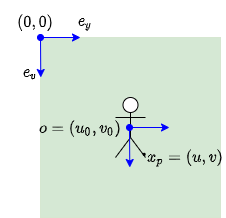
\includegraphics[width=.5\textwidth]{graphics/td_scene_xy.png}
    \caption{The pinhole camera model, x-y plane}
    \label{fig:td_scene_xy}
  \end{subfigure}
  \hfill
  \begin{subfigure}[b]{0.5\textwidth}
    \centering
    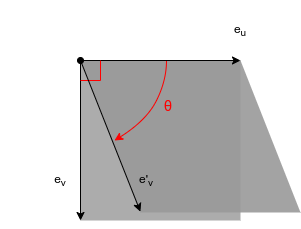
\includegraphics[width=.5\textwidth]{graphics/pixel.png}
    \caption{A scheme of a pixel skew}
    \label{fig:Kframes}
  \end{subfigure}
\end{figure}

In the physical implementation of the camera Obscura, the projective plane is on the opposite side from the projection center (or camera center $\vec{C}$ in the pinhole camera model), and the image is reversed and mirrored. 
However, in most computer vision literature, authors assume that it is on the same side as the object (see \autoref{fig:td_scene_3d}).
In \autoref{fig:td_scene_3d} a camera with camera center $C$ in a coordinate system with origin at $\vec{C}$ and basis vectors $(\vec{e}_x, \vec{e}_y, \vec{e}_z)$ is observing human. 
Each point $\vec{X} = (x, y, z)^\top$ in a world coordinate system has a projection $\vec{m} = (u, v)^\top$ on a plane $\pi$ which is located on a distance $f$ from the camera center (\autoref{fig:td_scene_yz}). 
The optical axis $\vec{O}$ is a ray perpendicular to plane $\pi$, and on the image the point $ \vec{O} \cap \pi = \vec{o}$ is the center of the image, see \autoref{fig:td_scene_xy}.

\subsection{Camera matrix}
The camera calibration matrix is a matrix that includes the camera's \textit{intrinsic} parameters - focal length, pixel skew angle ($\theta$), as on \autoref{fig:Kframes}, pixel aspect ratio \textit{a} and principle point coordinates $\vec{o} = (u_0, v_0)$ \autoref{fig:td_scene_xy}.
\begin{equation}
    \mat{K} = \begin{bmatrix}
        f_x & -a f \cot(\theta) & u_0 \\
        0 & f_y & v_0 \\
        0 & 0 & 1 \\
    \end{bmatrix} 
    \textrm{ ,units: } [f]=m, [u_0]=px, [v_0]=px, [a]=1,
\end{equation}

where $f_x = af$, $f_y = \frac{f}{\sin{\theta}}$, $f$ is a focal length used to convert world length ratios to pixels.

Most modern digital cameras have no skew and square pixels, so in most cases, the camera matrix can be simplified to:

\begin{equation}
    \label{eq:kmat}
    \pmb{\mathsf{K}} = \begin{bmatrix}
        f_x & 0 & u_0 \\
        0 & f_y & v_0 \\
        0 & 0 & 1 \\
    \end{bmatrix};
\end{equation}

\subsection{Projection matrix}

\begin{figure}[h]
    \centering
    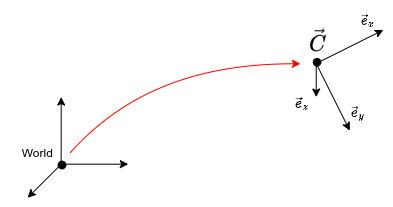
\includegraphics[width=.5\textwidth]{graphics/frames.png}
    \caption{Transformation from world to camera coordinate frames}
    \label{fig:frames}
\end{figure}

To translate a point from a world coordinate frame to an image coordinate frame, the Image projection matrix $\pmb{\mathsf{P}}$ is used. 
The canonical projection matrix $\pmb{\mathsf{P}}_0$ assumes that the camera is in the world coordinate center and that the calibration matrix $\pmb{\mathsf{K}} = \pmb{\mathsf{I}}$
\begin{equation}
\pmb{\mathsf{P}}_0 = \begin{bmatrix} \pmb{\mathsf{I}} & | & \vec{0} \end{bmatrix} = 
    \begin{bmatrix}
    1 & 0 & 0 & 0 \\
    0 & 1 & 0 & 0 \\
    0 & 0 & 1 & 0 \\
    \end{bmatrix};
\end{equation}

However, this case is impractical. 
The canonical projection matrix is not used in practice because each real camera is different. 
Instead, the image projection matrix $\mat{P}$ is used with a camera matrix $\mat{K}$ to transform canonical $\mat{P}_0$ to perspective $\mat{P}$:

\begin{equation}
\pmb{\mathsf{P}} = \pmb{\mathsf{K}} \begin{bmatrix} \pmb{\mathsf{I}} & | & \vec{0} \end{bmatrix} = 
    \begin{bmatrix} 
    f_x & 0 & u_0 & 0 \\
    0 & f_y & v_0 & 0 \\ 
    0 & 0 & 1 & 0 \\
    \end{bmatrix}.
\end{equation}

The world coordinate center is usually not located at point $\vec{C}$ (\autoref{fig:frames}). 
It may be rotated using a rotation matrix $\mat{R}$ and translated on vector $\vec{t}$ where $\mat{R}$ is a $3x3$ matrix with $det(\mat{R}) = 1$ and $\mat{R}^{-1} = \mat{R}^\top$. 
Therefor, in the general case the projection can be expressed as
\begin{equation}
    \pmb{\mathsf{P}} = \pmb{\mathsf{K}} \begin{bmatrix} \pmb{\mathsf{R}} & | & \vec{t} \end{bmatrix} = 
    \pmb{\mathsf{K}} \begin{bmatrix} \pmb{\mathsf{R}} & | & - \pmb{\mathsf{R}} \pmb{\mathsf{C}} \end{bmatrix},
\end{equation}

where $\vec{C}$ is the camera's position in a world reference frame. 

Image point $\vec{m} = (u, v)^\top$ can be obtained from a 3D point $\vec{X}$ using the projection matrix $\mat{P}$ as

\begin{equation}
    \label{eq:projection}
    \lambda \begin{bmatrix} 
        u \\ v \\ 1 \end{bmatrix} = \pmb{\mathsf{P}} \begin{bmatrix} x \\ y \\ z \\ 1
    \end{bmatrix},
\end{equation}

\begin{equation}
    \lambda \begin{bmatrix} 
    \vec{m} \\ 1 \end{bmatrix} = \pmb{\mathsf{P}} \begin{bmatrix} \vec{X} \\ 1
\end{bmatrix},
\end{equation}
where $\lambda \neq 0$ is a free scaling parameter.

\section{Epipolar geometry}

\subsection{Skew-symmetric 3x3 matrix}
A skew-symmetric or antisymetric matrix is such matrix $[\vec{b}]_{\times}$ that $[\vec{b}]_{\times}^\top = -[\vec{b}]_{\times}$. 
For vector $\vec{b} = (b_1, b_2, b_3)^\top$:
\begin{equation}
    [\vec{b}]_{\times} = \begin{bmatrix}
        0 & -b_3 & b_2 \\ 
        b_3 & 0 & b_1 \\ 
        -b_2 & b_1 & 0 \\ 
    \end{bmatrix};
\end{equation}

This matrix has some essential properties, but the most important in this thesis - it generalizes across a product as matrix multiplication.
\begin{equation}
    \vec{a} \times \vec{b} = [\vec{a}]_{\times} \vec{b};
\end{equation}
Notation is taken from \cite{hartley_zisserman_2004}, p. 581.
\subsection{Epipolar geometry}
\label{epipolar_geometry}
\begin{figure}[h]
    \centering
    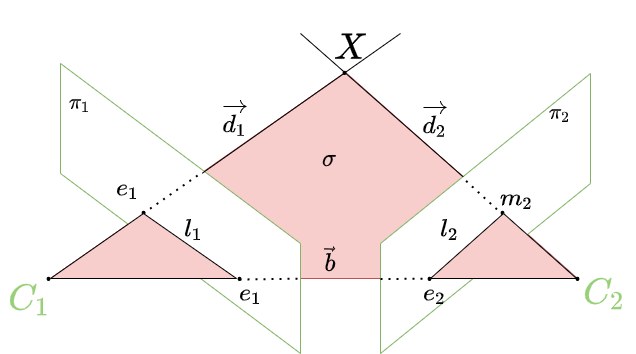
\includegraphics[width=0.9\textwidth]{graphics/epipolar.png}
    \caption{Epipolar geometry scheme}
    \label{fig:epipolar_std}
\end{figure}

\autoref{fig:epipolar_std} shows a scheme of two cameras with different camera centers $\vec{C}_1$ and $\vec{C}_2$ connected with a base line $\vec{b} = \vec{C}_2 - \vec{C}_1$. 
Both of them are seen as some 3d point $X$. 
This point projections are $\vec{m}_1$ and $\vec{m}_2$ respectivly. 
Points $\vec{C}_1, \vec{C}_2$ and $\vec{X}$ form an \textit{epipolar plane} $\sigma$.
$\sigma \cap \pi_1 = \vec{l}_1$ and $\sigma \cap \pi_2 = \vec{l}_2$ are images of \textit{epipolar lines}. 
Epipolar line $\vec{l}_1$ passes through \textit{epipole} $\vec{e}_1$, where $\lambda [\vec{e}_1 | 1]^\top = \pmb{\mathsf{P}}_2 \vec{C}_1$, same with $\lambda [\vec{e}_2 | 1]^\top = \pmb{\mathsf{P}}_1 \vec{C}_2$.

\subsection{Epipolar constraint}

Having a set of two cameras the relationship between them and constraints on them can be expressed by two new matrices \textit{Essential matrix} $\pmb{\mathsf{E}} \in \mathbb{R}^{3x3}, rank(\pmb{\mathsf{E}}) = 2$, \autoref{eq:E} and \textit{Fundamental matrix} $\pmb{\mathsf{F}} \in \mathbb{R}^{3x3}, rank(\pmb{\mathsf{F}}) = 2$, \autoref{eq:F}
\begin{equation}
    \label{eq:E}
    \pmb{\mathsf{E}} = \pmb{\mathsf{R}}_2 [\vec{C}_2 - \vec{C}_1]_{\times} \pmb{\mathsf{R}}_1^\top = [-\vec{t}_{21}]_{\times} \pmb{\mathsf{R}}_{21} = [\vec{b}]_{\times} \pmb{\mathsf{R}}_{21};
\end{equation}
\begin{equation}
    \label{eq:F}
    \pmb{\mathsf{F}} = \pmb{\mathsf{K}}_2^{-T} \pmb{\mathsf{R}}_2 [\vec{C}_2 - \vec{C}_1]_{\times} \pmb{\mathsf{R}}_1^\top \pmb{\mathsf{K}}_1^{-1} = 
    \pmb{\mathsf{K}}_2^{-T} [-\vec{t}_{21}]_{\times} \pmb{\mathsf{R}}_{21} \pmb{\mathsf{K}}_1^{-1} = 
    \pmb{\mathsf{K}}_2^{-T} \pmb{\mathsf{E}} \pmb{\mathsf{K}}_1^{-1};
\end{equation}
where 
$\pmb{\mathsf{R}}_{21} = \pmb{\mathsf{R}}_2 \pmb{\mathsf{R}}_1^\top$ is a relative camera rotation and 
$\vec{t}_{21} = -\pmb{\mathsf{R}}_2 \vec{b} = \vec{t}_2 - \pmb{\mathsf{R}}_{21}\vec{t}_1$ is a relative camera translation.

An algebraic expression of important properties of matrix $F$:
\begin{equation}
    \label{eq:Fm2}
    \lambda l_1 = \pmb{\mathsf{F}}^\top \begin{bmatrix} \vec{m}_2 \\ 1 \end{bmatrix},
\end{equation}
\begin{equation}
    \label{eq:Fm1}
    \lambda l_2 = \pmb{\mathsf{F}} \begin{bmatrix} \vec{m}_1 \\ 1 \end{bmatrix},
\end{equation}
\begin{equation}
    \label{eq:fefe}
    \pmb{\mathsf{F}} \begin{bmatrix} \vec{e}_1 \\ 1 \end{bmatrix} = \pmb{\mathsf{F}}^\top \begin{bmatrix} \vec{e}_2 \\ 1 \end{bmatrix} = 0,
\end{equation}
\begin{equation}
    \label{eq:epiconstr}
    \begin{bmatrix} \vec{m}_2 & | & 1 \end{bmatrix} \pmb{\mathsf{F}} \begin{bmatrix} \vec{m}_1 \\ 1 \end{bmatrix} = 0.
\end{equation}
Matrix $\pmb{\mathsf{F}}$ maps points from $\pi_1$ to epipolar lines on $\pi_2$ and vice versa (\autoref{eq:Fm2} and \autoref{eq:Fm1}); epipoles $\vec{e}_1$ and $\vec{e}_2$ are right and left nullspaces basis vectors of $\pmb{\mathsf{F}}$ respectivly (\autoref{eq:fefe}).
Epipolar constraint \autoref{eq:epiconstr} means that a point and its corespondent line are on a same plane (\autoref{fig:epipolar_std}, plane $\sigma$).

\section{Stereovision}

\begin{figure}[h]
    \centering
    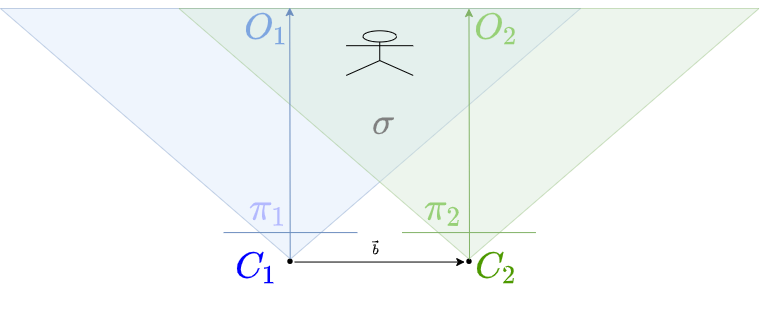
\includegraphics[width=0.7\textwidth]{graphics/stereopair.png}
    \caption{A stereovision scheme}
    \label{fig:sch_stereo}
\end{figure}
\begin{figure}[h]
    \centering
    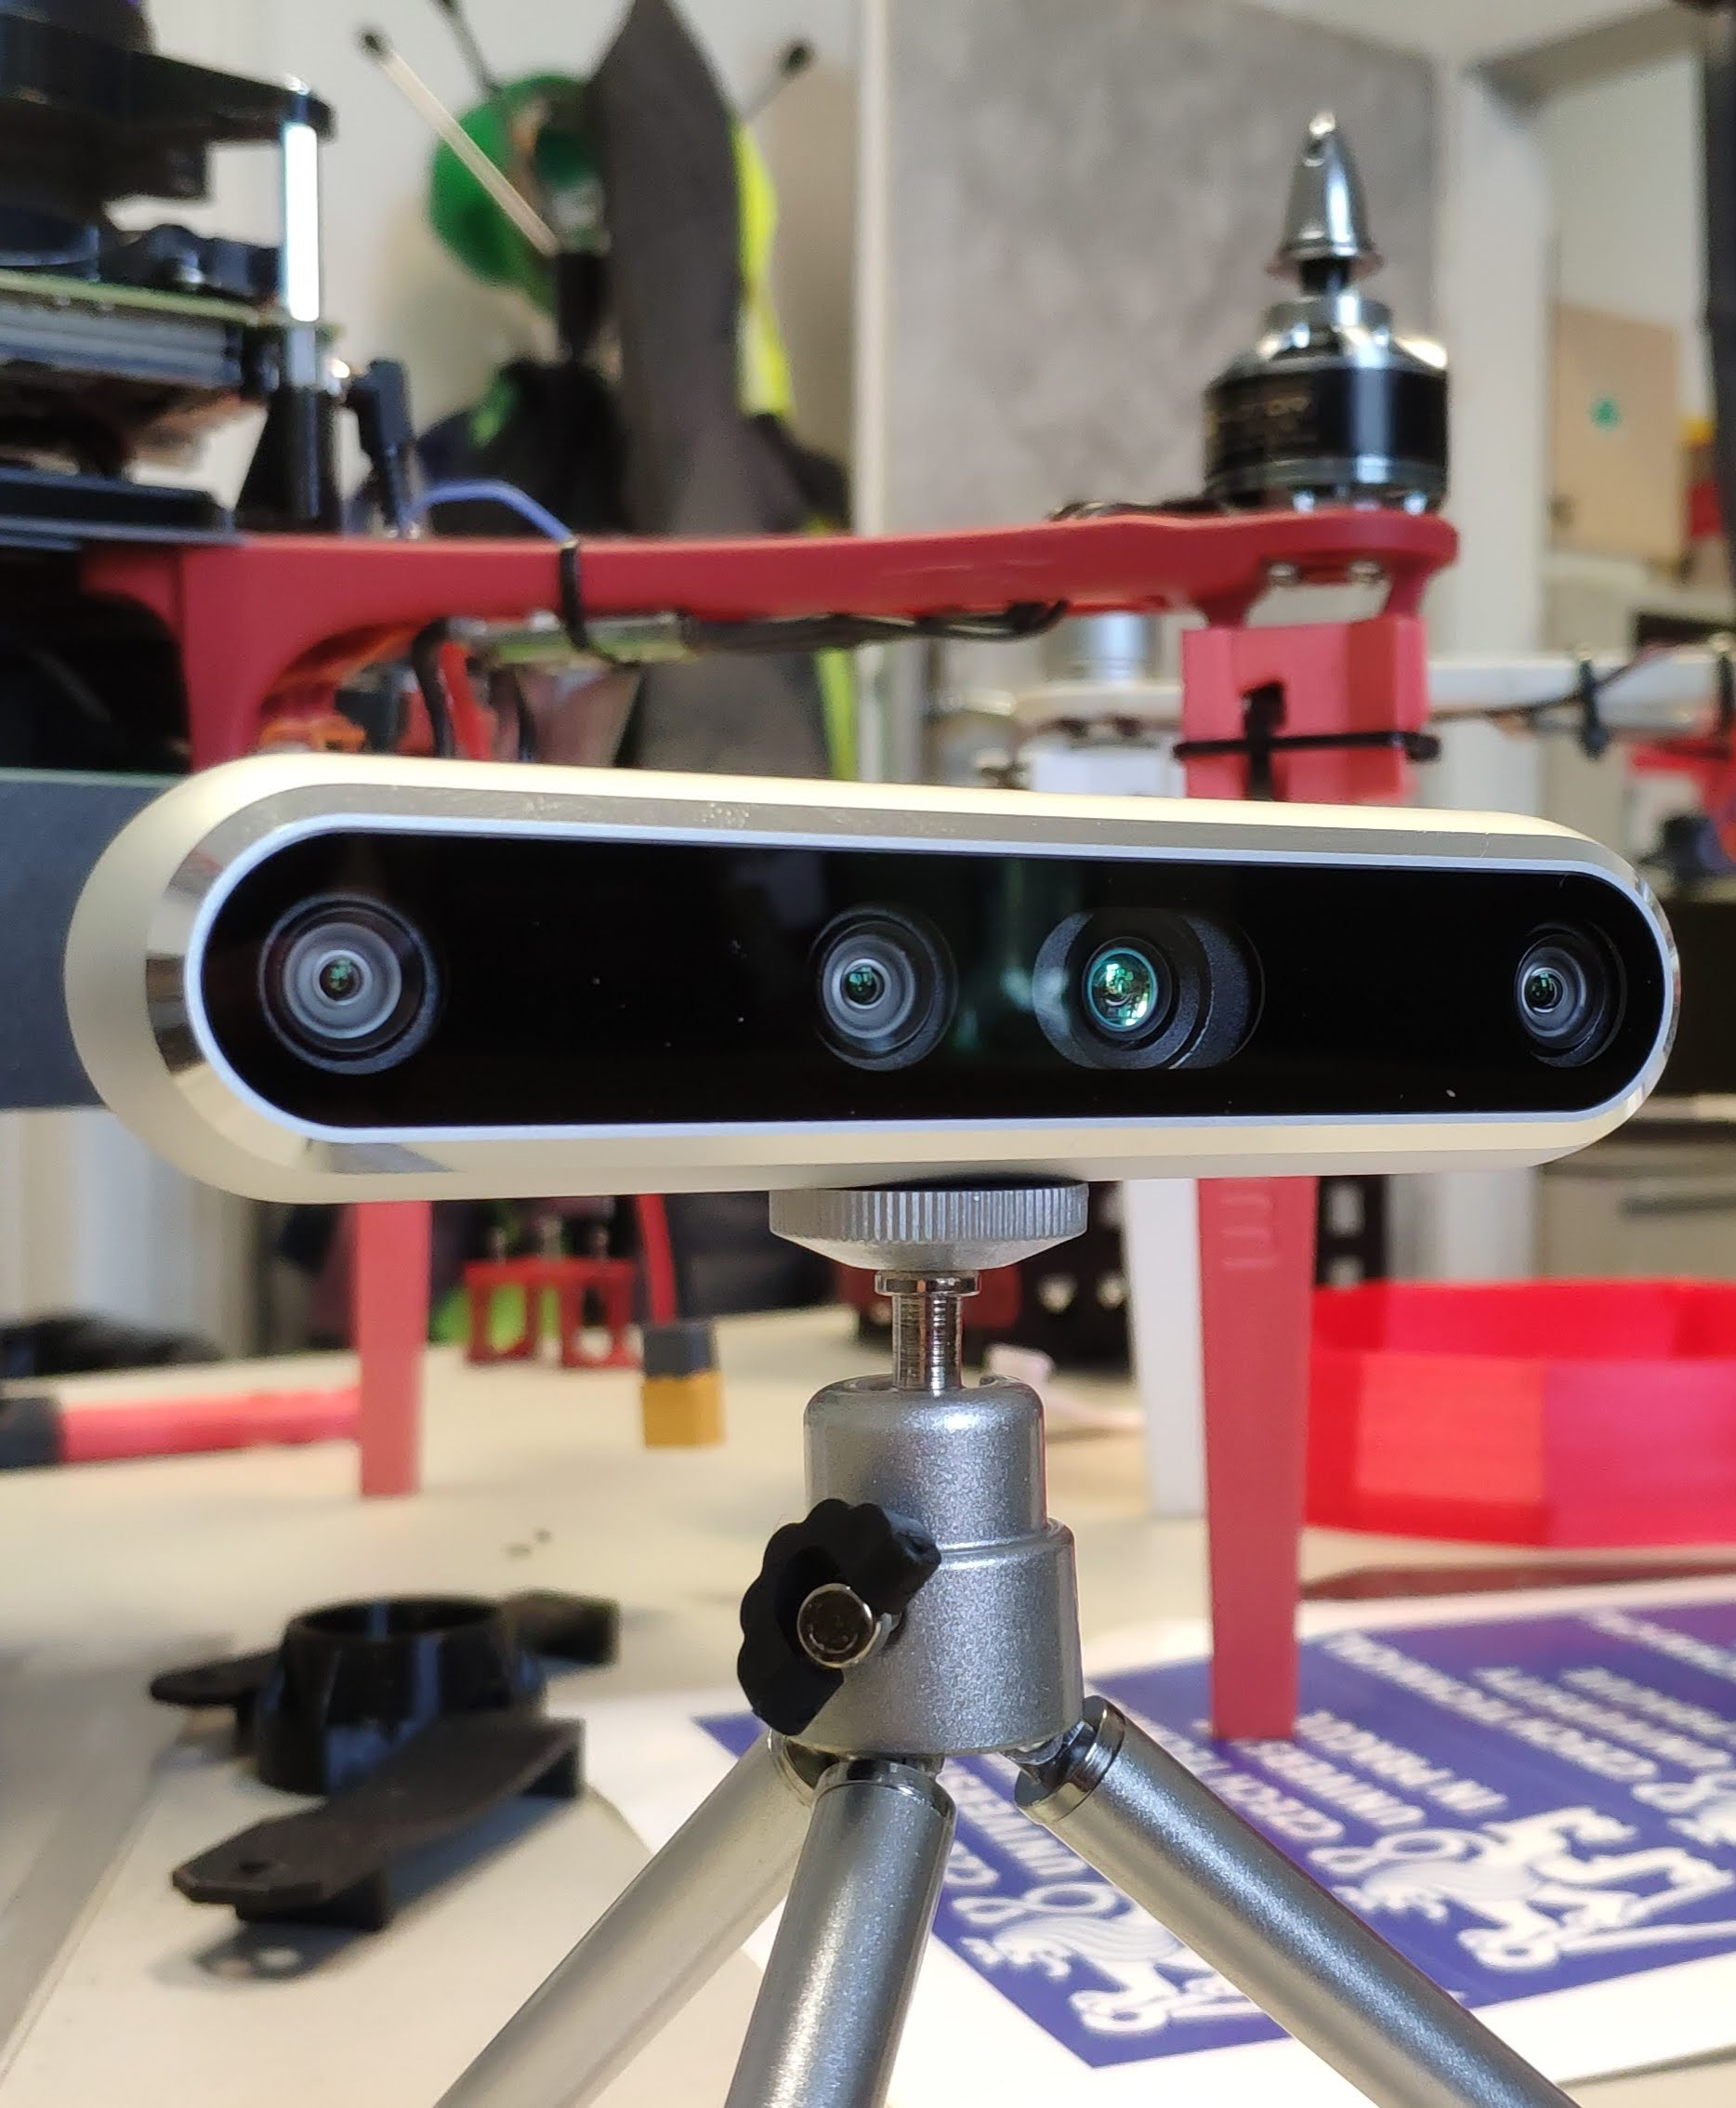
\includegraphics[width=0.3\textwidth]{graphics/stereo_example.jpg}
    \caption{Industrial stereocamera example, Intel realsense D455}
    \label{fig:stereo_ex}
\end{figure}

\begin{figure}[h]
    \begin{subfigure}[b]{0.31\textwidth}
      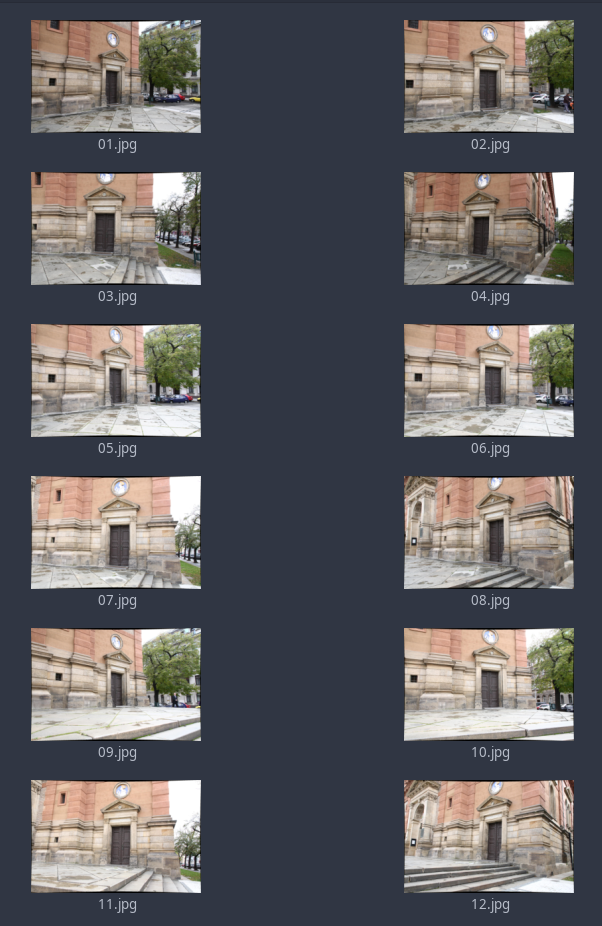
\includegraphics[width=\textwidth]{graphics/input_set.png}
      \caption{Input set of images.}
      \label{fig:pc_input}
    \end{subfigure}
    \hfill
    \begin{subfigure}[b]{0.65\textwidth}
      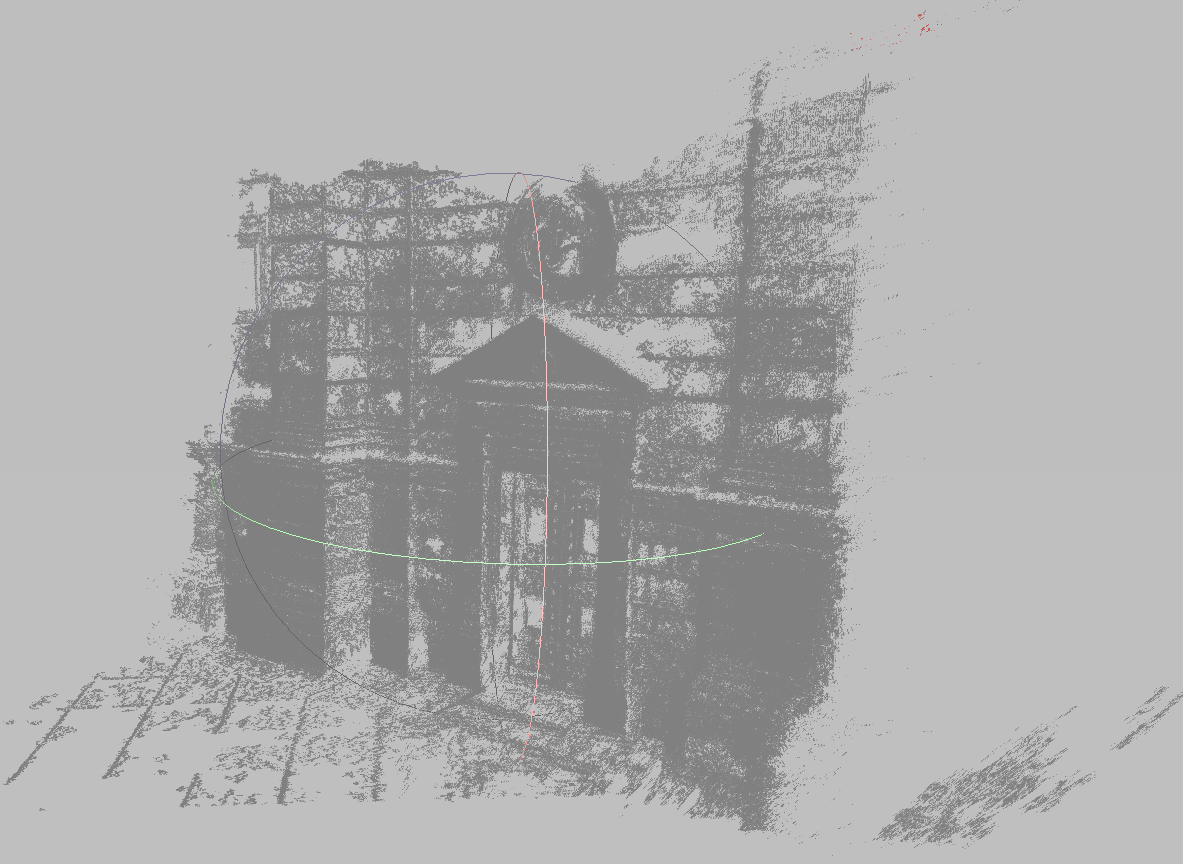
\includegraphics[width=\textwidth]{graphics/reconstructed.png}
      \caption{reconstructed pointcloud.}
      \label{fig:pc_output}
    \end{subfigure}
    \caption{Three dimensional reconstruction from multiple cameras.}
    \label{fig:pc_recons}
\end{figure}

Computer stereo vision is a process of extracting a stereo (depth) image from a planar image or set of images of the same scene. Usually, a stereo camera has two simple cameras located at some distance $\vec{b}$ pointing in the same direction, the same as the human eye (the scheme \autoref{fig:sch_stereo} and an example of a stereo camera \autoref{fig:stereo_ex}). 
Sometimes fusion of multiple cameras and other sensors can be used:
Intel Realsense \autoref{fig:stereo_ex} has two cameras, an IR sensor in case the images have almost no texture and a color sensor. 

\begin{equation}
    \label{eq:e1e2}
    \vec{e}_1 = \vec{e}_2 = \lambda \begin{bmatrix} 1 \\ 0 \\ 0 \end{bmatrix};
\end{equation}
\begin{equation}
    \label{eq:e1m1}
    \lambda \vec{l}_1 = \vec{e}_1 \times \vec{m}_1 = [\vec{e}_1]_\times \begin{bmatrix} \vec{m}_1 \\ 1\end{bmatrix};
\end{equation}
\begin{equation}
    \label{eq:F_simple}
    \pmb{\mathsf{F}} = \lambda [\vec{e}_1]_\times = \lambda \begin{bmatrix}
        0 & 0 & 0 \\
        0 & 0 & -1 \\
        0 & 1 & 0 \\
    \end{bmatrix};
\end{equation}

It is possible to calculate only the non-zero multiple of $\mat{E}$ from image correspondences so that the scene can be reconstructed only up to a scale, but knowing the translation vector $\vec{b}$ (\autoref{fig:sch_stereo}), means having a calibrated stereo pair, all distances can be calculated in world coordinates frame.
By removing a rotation between cameras ($\mat{R} = \mat{I}$), all computations are simplified.

Corresponding epipolar lines lie on same image rows ($l_1 = l_2$), and intersects at "points at infinity" (\autoref{eq:e1e2}). 
Epipole is a point of intersecting all epipolar lines, so having the intersecting point ($\vec{e}_1$) and image point epipolar line can be calculated (\autoref{eq:e1m1}), therefore considering \autoref{eq:Fm1}, \autoref{eq:e1e2} and \autoref{eq:e1m1} the \autoref{eq:F_simple} is true.

Consider two correspondences $\vec{a}_1 = (u_1, v)^\top$ and $\vec{a}_2 = (u_2, v)^\top $. 
Having correspondent points on the same row means that feature matcher can use this correlation to accelerate a matching process.
It is possible to receive a dense point cloud as on \autoref{fig:pc_output} with this approach.

\section{Calibration}
\label{sec:prelimin_calibration}
\subsection{Single camera calibration}

\begin{figure}[h]
    \centering
    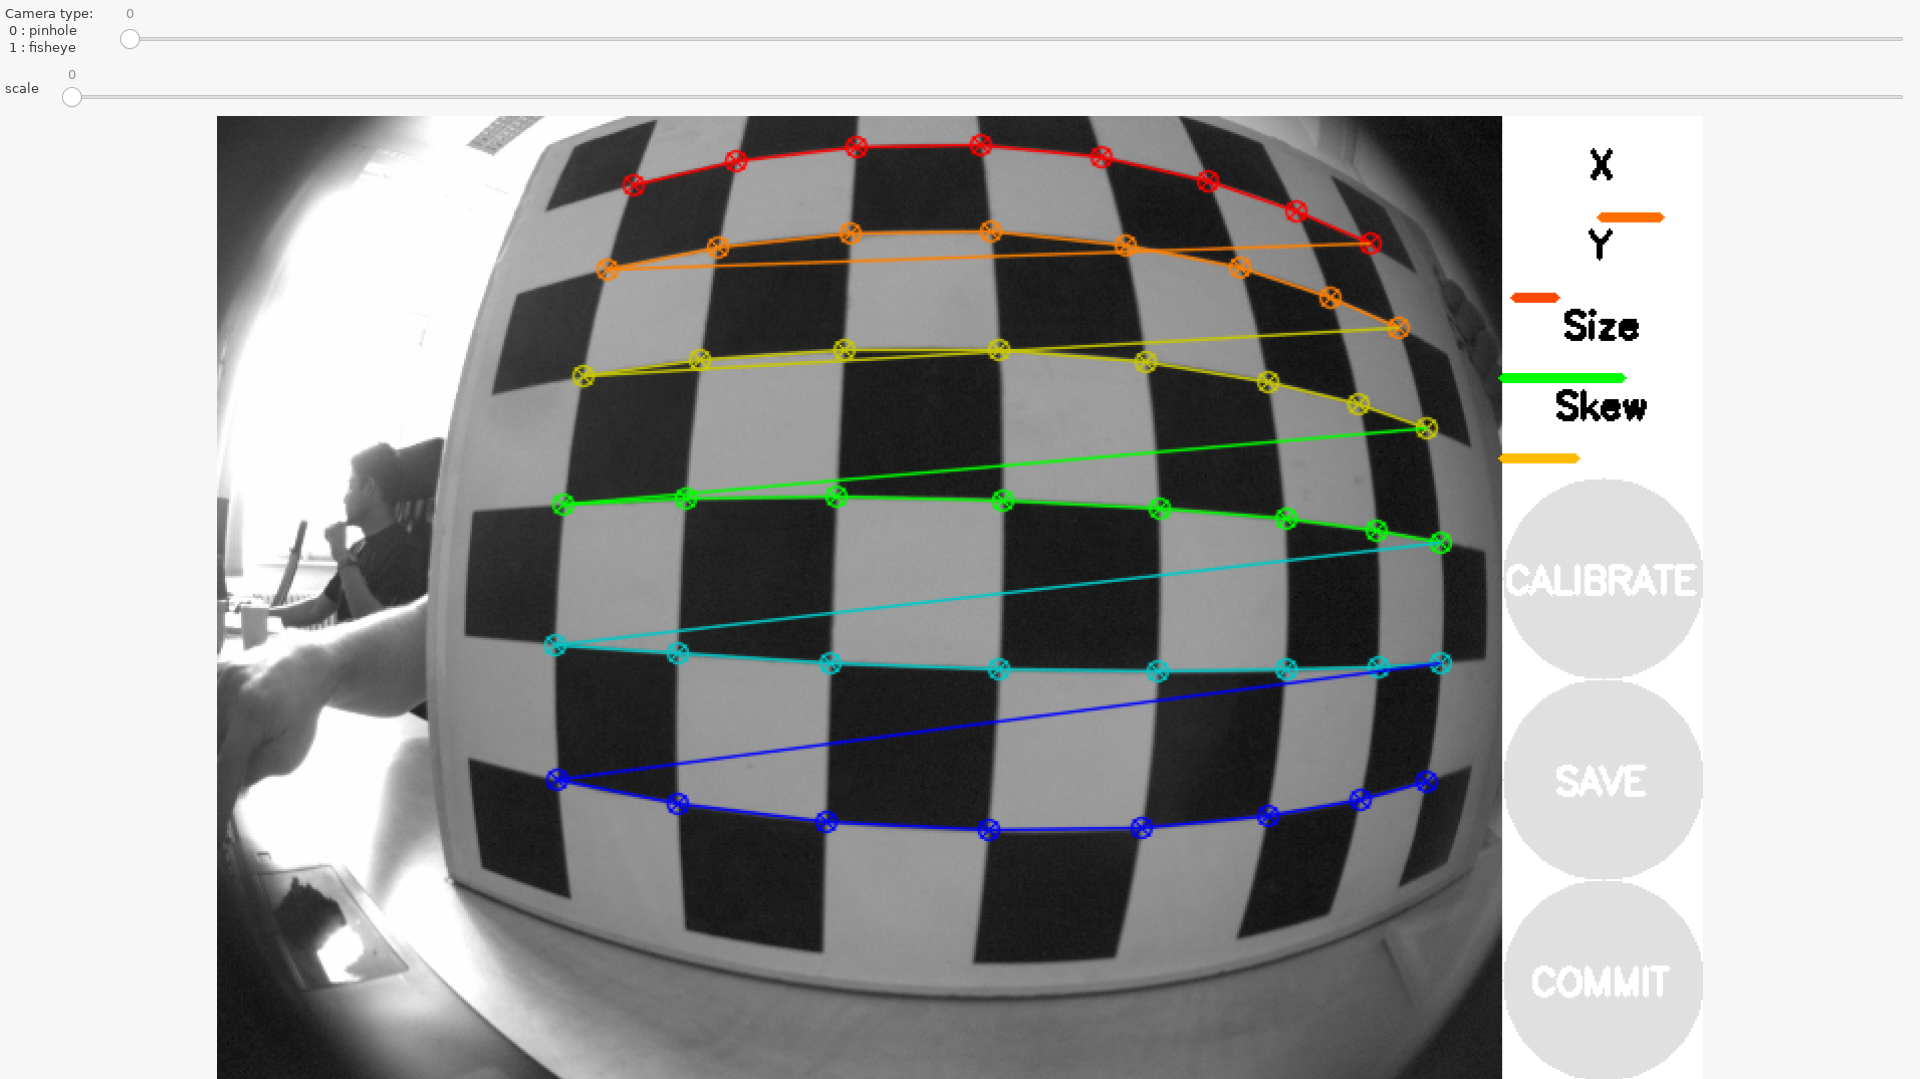
\includegraphics[width=.6\textwidth]{graphics/calibration.png}
    \caption{Calibration process}
    \label{fig:calib}
\end{figure}

\begin{figure}[h]
    \begin{subfigure}[b]{0.45\textwidth}
      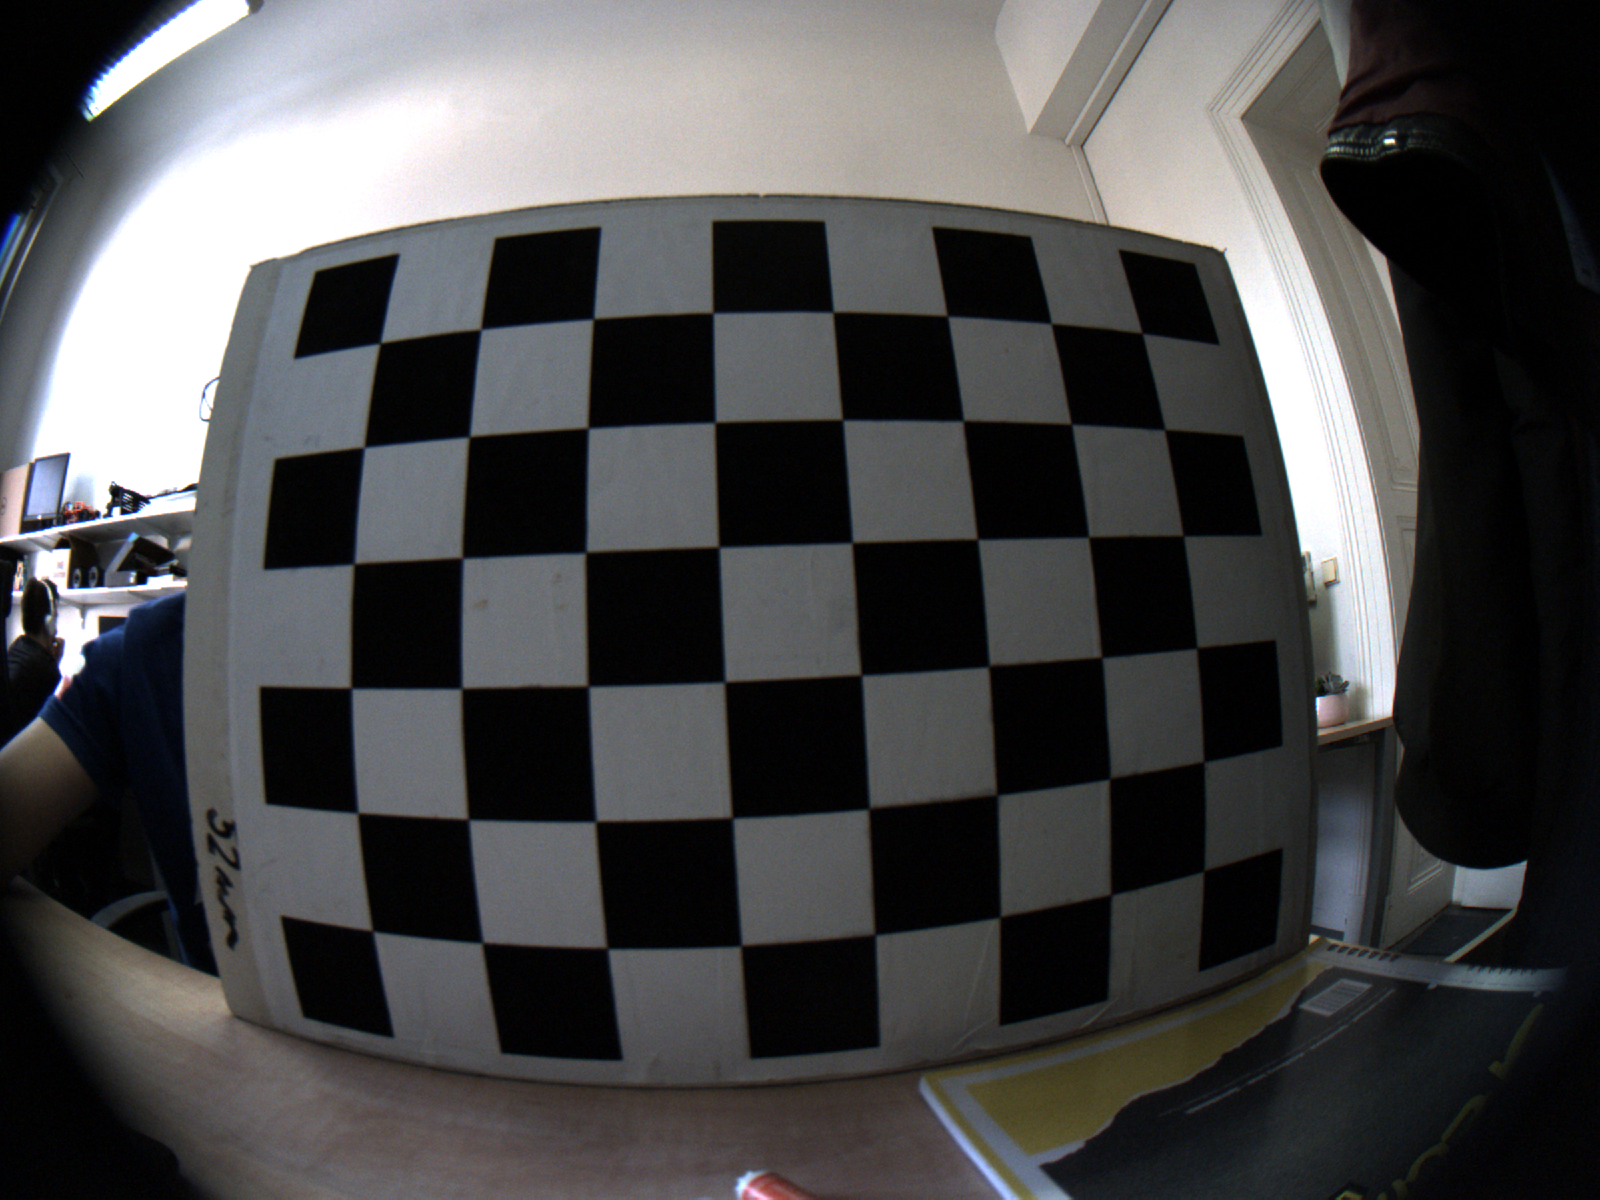
\includegraphics[width=\textwidth]{graphics/chessboard_img.png}
      \caption{Original image with radial distortion.}
      \label{fig:chb1}
    \end{subfigure}
    \hfill
    \begin{subfigure}[b]{0.45\textwidth}
      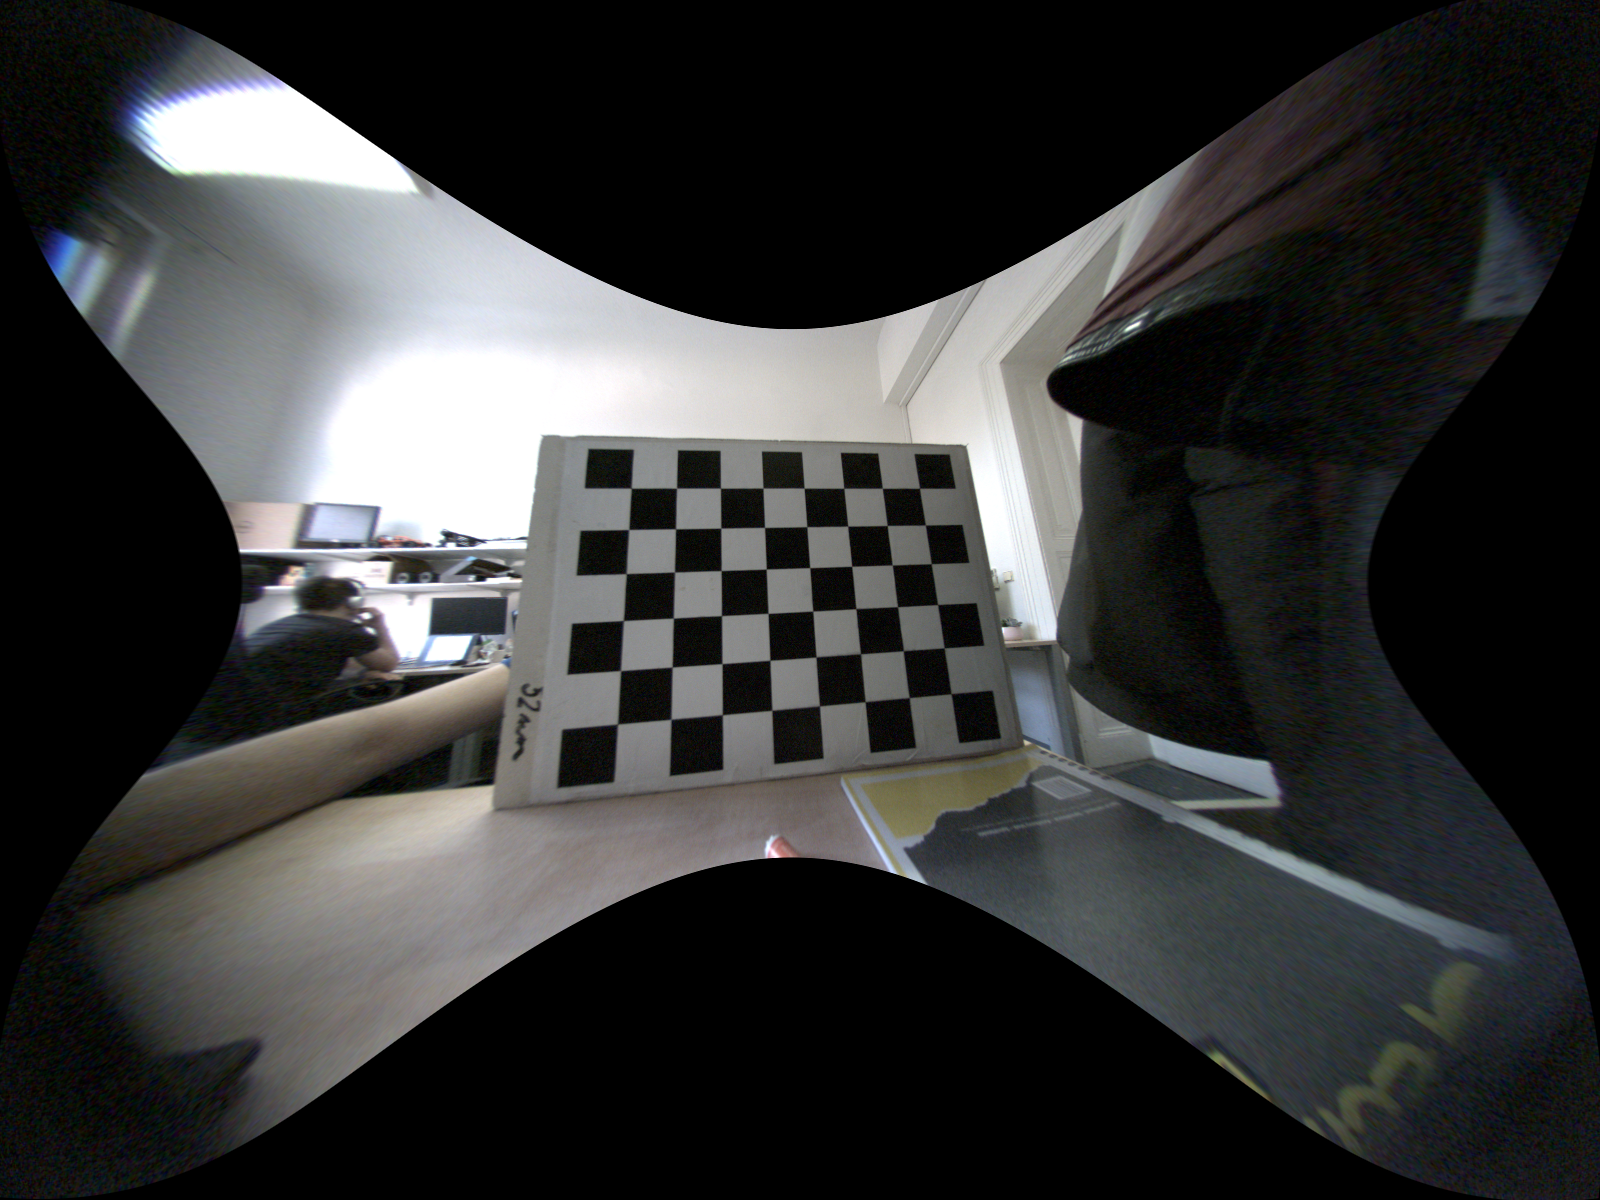
\includegraphics[width=\textwidth]{graphics/chessboard_img_rect.png}
      \caption{Undistorted image with no distortion.}
      \label{fig:chb2}
    \end{subfigure}
    \caption{Camera image before and after the calibration}
    \label{fig:chb}
\end{figure}

Camera calibration - or \textit{Camera resection} process of computing the camera calibration matrix $K$ (\autoref{eq:kmat}).
Usually, it is done with some pattern with predefined parameters, like a chessboard or more advanced boards (ArUco and ChArUco\footnote{\href{https://docs.opencv.org/4.x/df/d4a/tutorial_charuco_detection.html}{Opencv ChArUco and ArUco boards}}).

Camera calibration is necessary for geometry correction (\autoref{fig:chb}), so as a result, parallel lines in 3D are parallel to the image after the undistortion, and the image is unwrapped and projected on a plane.

In a real world lenses has also some distortion (\autoref{fig:chb1}) so to fix that distortion coefficients should be calculated: radial distortion $k_1, k_2, k_3, k_4, k_5, k_6$ and tangential distortion $p_1, p_2$.

From the \autoref{eq:projection}:
\begin{equation}
    \label{eq:dist_start}
    \lambda \begin{bmatrix} 
        u \\ v \\ 1 \end{bmatrix} = \pmb{\mathsf{K}} [\pmb{\mathsf{R}} | \vec{t}] \begin{bmatrix} x \\ y \\ z \\ 1
    \end{bmatrix},
\end{equation}
\begin{equation}
    \label{eq:dist_2}
    \begin{bmatrix} x_c \\ y_c \\ z_c \end{bmatrix}
     = [\pmb{\mathsf{R}} | \vec{t}] \begin{bmatrix} x \\ y \\ z \\ 1
    \end{bmatrix},
\end{equation}
\begin{equation}
    \label{eq:dist_3}
    x'' = \frac{x_c}{z_c} \frac{1 + k_1r^2 + k_2r^4 + k_3r^6}{1 + k_4r^2 + k_5r^4 + k_6r^6} + p_1(r + 2x') + 2p_2\frac{x_c y_c}{z^2_c},
\end{equation}
\begin{equation}
    \label{eq:dist_4}
    y'' = \frac{y_c}{z_c} \frac{1 + k_1r^2 + k_2r^4 + k_3r^6}{1 + k_4r^2 + k_5r^4 + k_6r^6} + 2p_1(\frac{x_c y_c}{z_c^2}) + p_2(r + 2y'),
\end{equation}
where $x' = (\frac{x_c}{z_c})^2$; $y' = (\frac{y_c}{z_c})^2$; $r = x' + y'$. Then undistorted point will be
\begin{equation}
    \label{eq:dist_end}
    \begin{bmatrix} u \\ v \\ 1 \end{bmatrix} = \pmb{\mathsf{K}} \begin{bmatrix} x'' \\ y'' \\ 1 \end{bmatrix}.
\end{equation}

Considering \autoref{eq:kmat}, image of a point $X$ seen through the calibrated camera with projection matrix $P$ will look as in \autoref{eq:dist_start} - \autoref{eq:dist_end}. Firstly, the point is projected on an abstract projection plane (\autoref{eq:dist_2}), then undistorted (\autoref{eq:dist_3}, \autoref{eq:dist_4}) and finally transformed from metric system of abstract projection plane to an image coordinate system (\autoref{eq:dist_end}).

\subsection{Stereopair calibration}
\label{sec:prelimin_stereocalib}
Stereo pair calibration is a process of estimating the essential matrix $\mat{E}$ for a camera pair, which also can be computed from a relative rotation matrix $\mat{R}_{21}$ and a relative translation vector $\vec{t}_{21}$ of a camera pair.

\clearpage
\chapter{Methodology}

\label{chapter:methodology}

\begin{figure}[h]
    \centering
    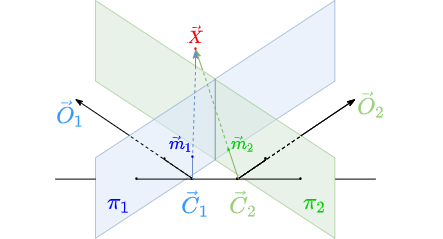
\includegraphics[width=.8\textwidth]{graphics/td90deg.png}
    \caption[The proposed approach model.]{Ilustration of the proposed approach. $\vec{C}_1$, $\vec{C}_2$ are optical centers of two cameras with projection plaes $\pi_1$ and $\pi_2$, $\vec{O}_1$ , $\vec{O}_2$ are the corresponding optical axes. The 3D point $\vec{X}$ is in the cameras' overlapping sone, $\vec{m}_1$ and $\vec{m}_2$ are its projections on corresponding image planes.}
    \label{fig:td90deg}
\end{figure}

The main task of this thesis is to create a compact obstacle avoidance system such that it can be mounted on MAVs with size and weight restrictions.
The proposed method is related to SfM or optical flow algorithms as well as standard stereo matching algorithms (see \autoref{fig:stereo_ex}).

Firstly, synchronized images from both cameras are captured. Features are detected using the feature extractor \autoref{sec:features} in the areas of these images that correspond to the overlapping part of their field of view. 
These features are then matched using the brute-force matcher.
The 3D position of each of these features relative to the cameras is estimated using a calibrated projection model and known relative transformation between the cameras.
Finally, the obtained 3D positions are the output of this algorithm. 

Quality of the 3D point estimation depends on the calibration of the cameras' relative transformation, the calibration of their projection model, the key point extractor and the matcher.
The obtained 3D points can be used to estimate the scale in an SfM algorithm that runs parallel to to the described method (refer to  \autoref{fig:intro_general}).
The estimated distance to nearby objects can be used in a feedback loop inside the system to correct path planning, considering the obstacles found.

This chapter describes the mathematical model of the problem and all algorithms used in the process: calibration of the projection model, calibration of the relative transformation between the cameras, feature extruction, feature matching and estimation of the 3D position of the matched features.

\section{Description of the optical setup}

The optical setup assumed by the proposed method shown in \autoref{fig:td90deg}.
There are two cameras with optical centers at $C_1$ and $C_2$ with a known static translation $\vec{t}_{21}$ and rotation $\mat{R}_{21}$ between coordinate frames of the cameras.
The rotation represented by $\mat{R}_{21}$ is assumed to be close to $90^\circ$ rotation in the epipolar plane (marked as $\sigma$ in \autoref{fig:epipolar_std}).
As described in \autoref{sec:problem_definition}, parameters of the mathematical projection model of the two cameras are assumed to be known. 
In practice, these are obtained using a calibration process, that is described in the next section.
Furthermore, it is assumed that the images coming from the cameras are synchronized and that the FOVs of both cameras have an intersecting zone.
Let us denote images from the two cameras as $i_1$ and $i_2$, a point in the environment $\vec{X}$ and its images in the two cameras $\vec{m}_1$ in image $i_1$ and $\vec{m}_2$ in image $i_2$.

\section{Projection model of a camera and its calibration}
\label{sec:meth_calib}
\begin{figure}[h]
    \begin{subfigure}[t]{0.45\textwidth}
      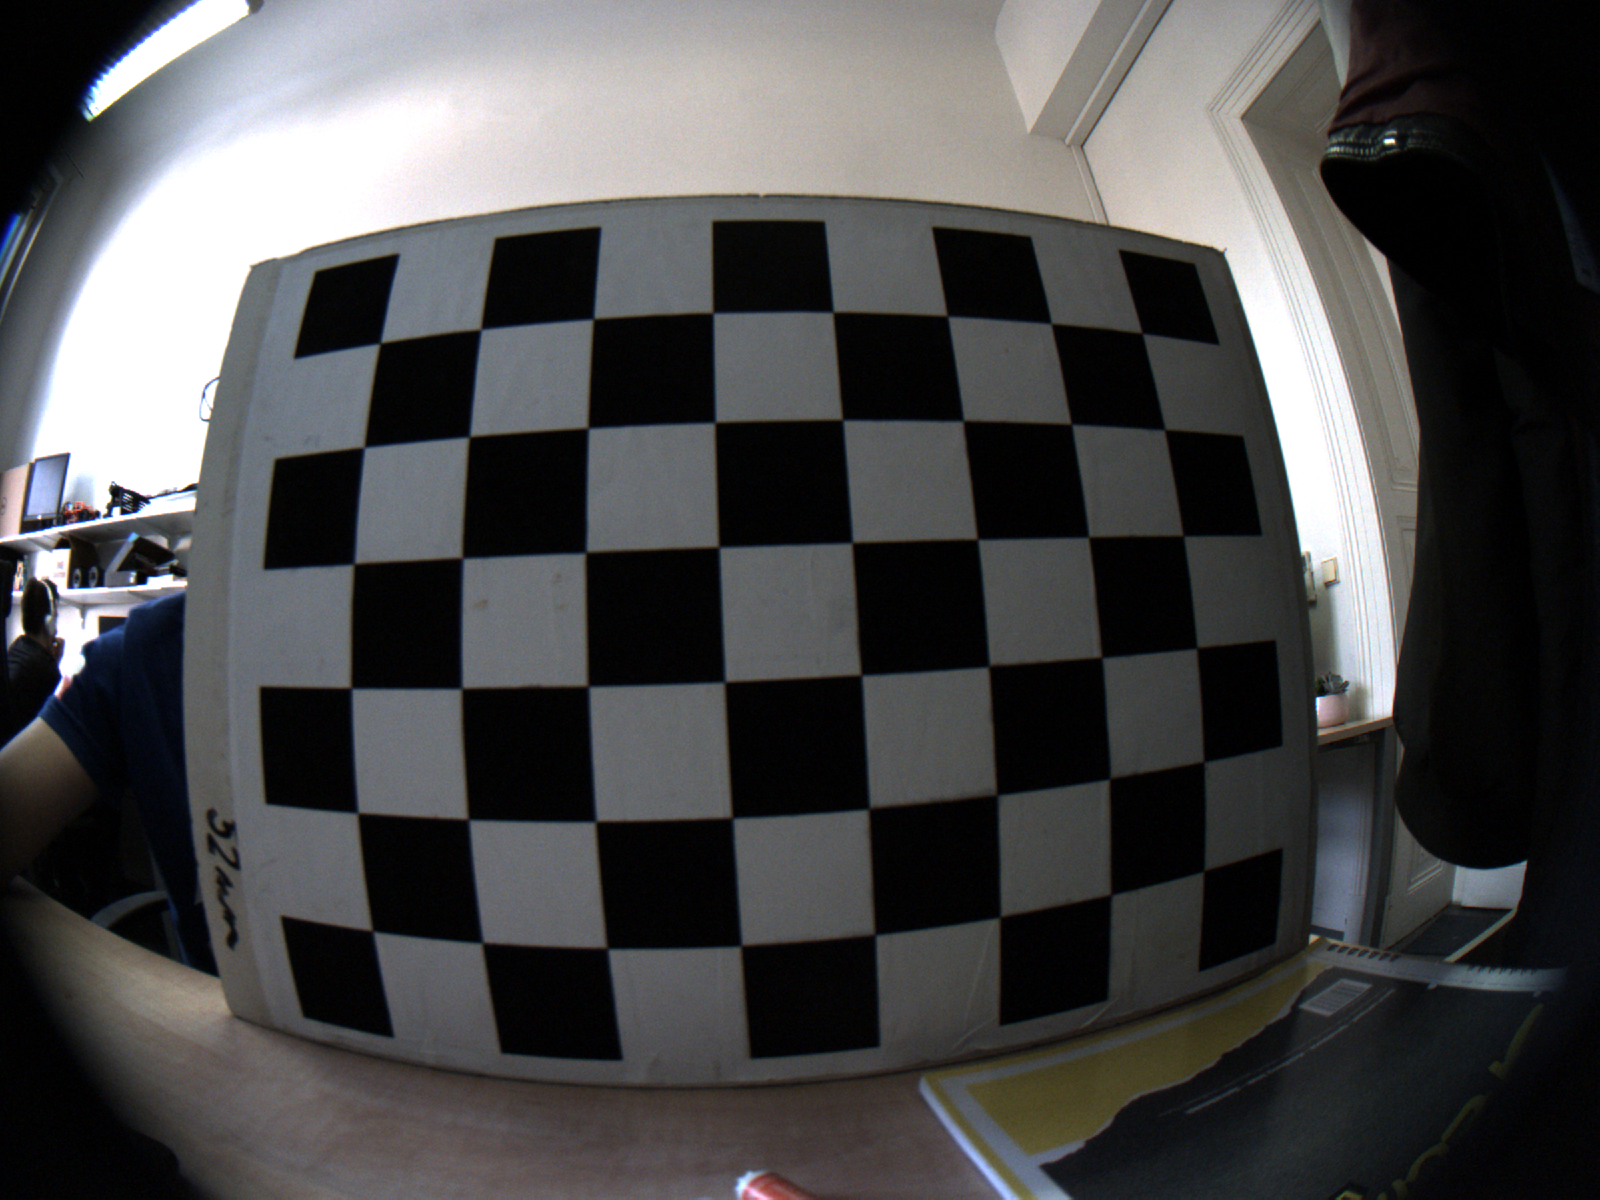
\includegraphics[width=\textwidth]{graphics/chessboard_img.png}
      \caption{Original image with radial distortion. Objects with straight edges appear curved in the image due to the distortion.}
      \label{fig:chb1}
    \end{subfigure}
    \hfill
    \begin{subfigure}[t]{0.45\textwidth}
      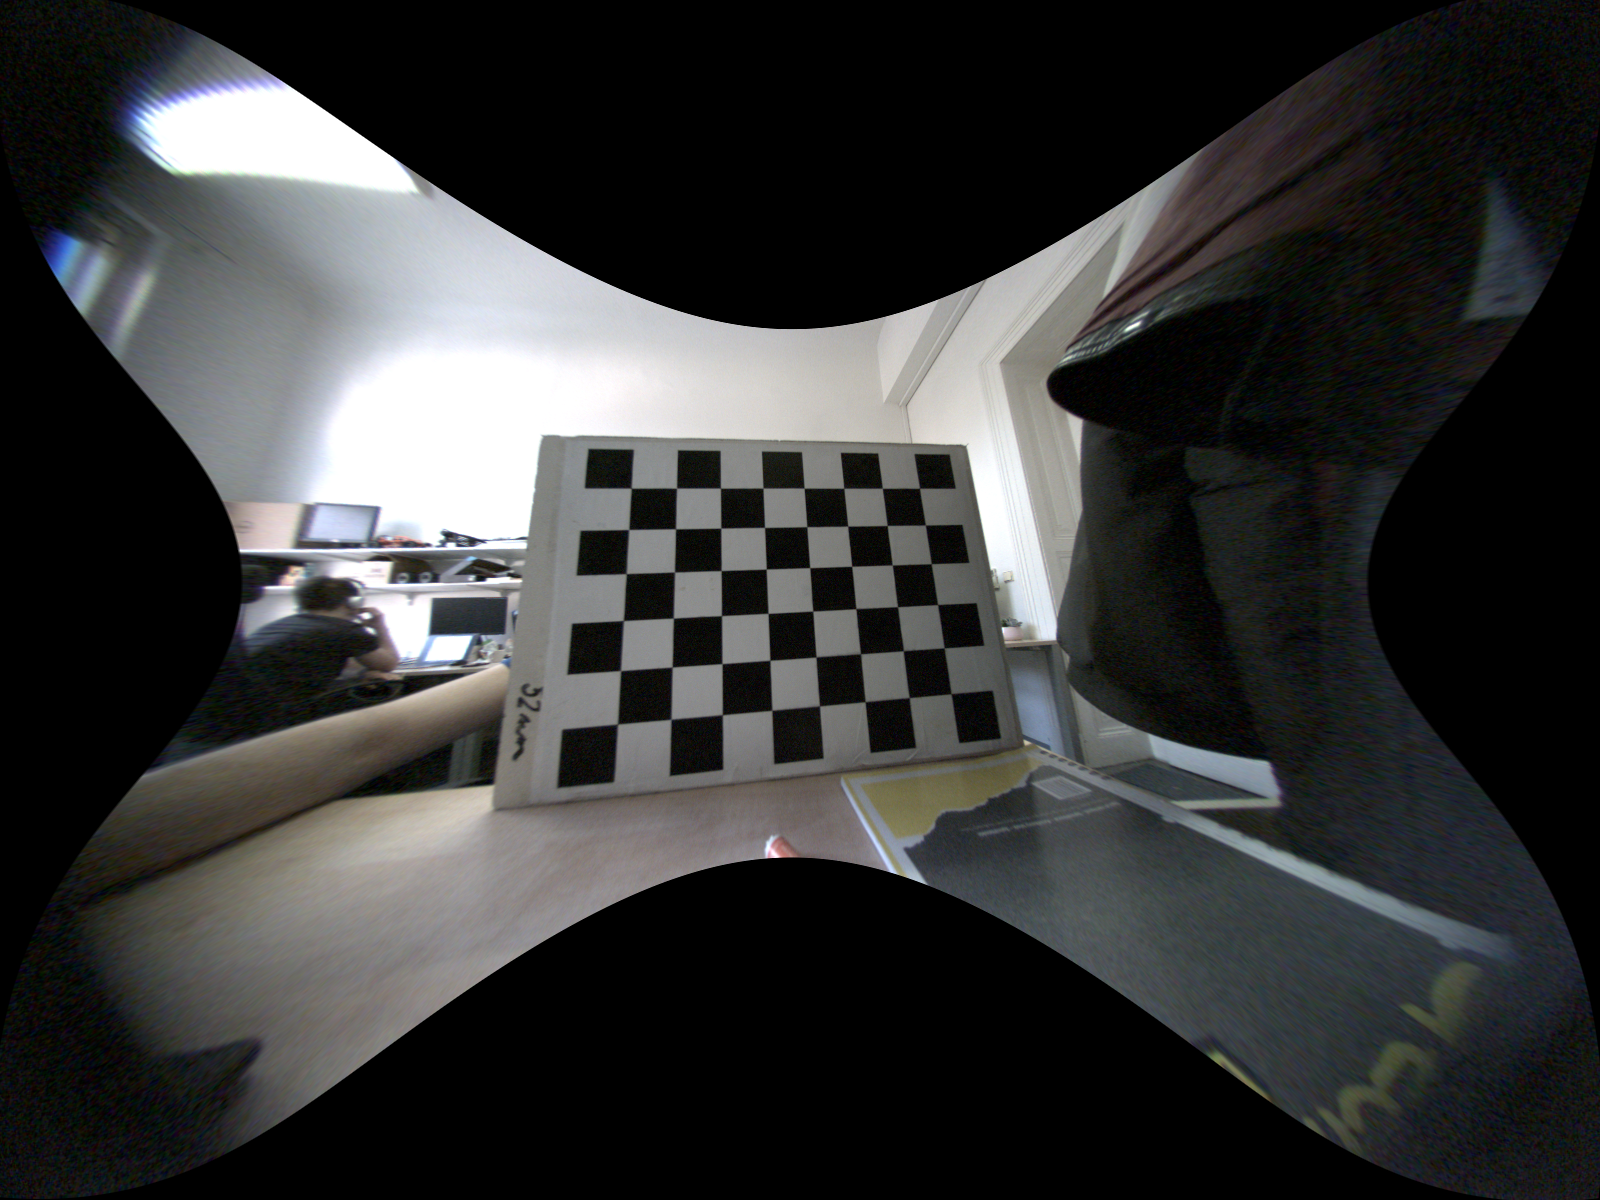
\includegraphics[width=\textwidth]{graphics/chessboard_img_rect.png}
      \caption{Image with no distortion. Edges that are straight in 3D are straight in the image.}
      \label{fig:chb2}
    \end{subfigure}
    \caption{An image from the camera before and after applying undistortion.}
    \label{fig:chb}
\end{figure}

Camera calibration is the process of empirically estimating the camera calibration matrix $\mat{K}$ (refer to \eqref{eq:kmat}) and distortion parameters of the camera's optical system for the pinhole camera model described in \autoref{sec:pinhole_camera_model}.
Usually, this is done with some pattern with predefined parameters, like a chessboard or more advanced markers (ChArUco and ArUco \cite{aruco} etc).

The camera calibration is necessary for geometrical image correction, distortion elimination, obtaining metric information and further estimating of distance (see \autoref{fig:chb}). 

In the real world, lenses have distortion (see \autoref{fig:chb1}).
To compensate that distortion, a polynomial model is often used with coefficients $k_1, ... , k_6$ for radial distortion and $p_1, p_2$ for tangential distortion.

\subsection{The minimal problem for camera calibration.} 
It is the problem of obtaining a projection matrix $\mat{P}$ given $n=6$ correspondences of 3D scene points and 2D image points $\{(\vec{X}_i, \vec{m}_i)\}_{i=1}^n$.
Let the projection matrix $\mat{P}$ be 
\begin{equation}
    \label{eq:p_calib}
    \mat{P} = \begin{bmatrix}
        \vec{q}_1^\top & q_{14} \\
        \vec{q}_2^\top & q_{24} \\
        \vec{q}_3^\top & q_{34} \\
    \end{bmatrix}.
\end{equation}

Then the equation \eqref{eq:proj_min} can be expanded to
\begin{equation}
    \lambda_i u_i = \vec{q}_1^\top \vec{X}_i + q_{14}, \;\;\;
    \lambda_i v_i = \vec{q}_2^\top \vec{X}_i + q_{24}, \;\;\;
    \lambda_i = \vec{q}_3^\top \vec{X}_i + q_{34}, \;\;\;
\end{equation}
where $\vec{m}_i = \begin{bmatrix} u_i \\ v_i \end{bmatrix}$, $ \lambda \in \mathbb{R}^{+}$, $i \in \{1, 2, ..., 6\}$.
After elimination of $\lambda_i$, we obtain
\begin{equation}
    (\vec{q}_3^\top \vec{X}_i + q_{34})u_i = \vec{q}_1^\top \vec{X}_i + q_{14},
\end{equation}
\begin{equation}
    (\vec{q}_3^\top \vec{X}_i + q_{34})v_i = \vec{q}_2^\top \vec{X}_i + q_{24}.
\end{equation}

Then
\begin{equation}
    \label{eq:Aqmat}
    \mat{A} \vec{q} = \begin{bmatrix}
        \vec{X}_1^\top & 1 & \vec{0}^\top & 0 & -u_1 \vec{X}_1^\top & -u1 \\
        \vec{0}^\top & 0 & \vec{X}_1^\top & 1 & -v_1 \vec{X}_1^\top & -v_1 \\ 
        \vdots & \vdots & \vdots & \vdots & \vdots & \vdots \\
        \vec{X}_k^\top & 1 & \vec{0}^\top & 0 & -u_k \vec{X}_k^\top & -uk \\
        \vec{0}^\top & 0 & \vec{X}_k^\top & 1 & -v_k \vec{X}_k^\top & -v_k \\ 
    \end{bmatrix} \begin{bmatrix}
        \vec{q}_1 \\ q_{14} \\ \vec{q}_2 \\ q_{24} \\ \vec{q}_3 \\ q_{34}
    \end{bmatrix} = \vec{0},
\end{equation}
so for $k=6$, $\mat{A} \in \mathbb{R}^{12 \times 12}$, $\vec{q} \in \mathbb{R}^{12}$. If $\mat{A}$ has rank 12, there is no non-trivial null space for $\mat{A}$.

\autoref{eq:Aqmat} can be solved by the so-called \textit{Jack-Knife estimation}. 
Let us denote a matrix $\mat{A}$ with the $i$-th row removed as $\mat{A}_i$. 
The \textit{Jack-Knife estimation} iterates through $i = 1, \dots, 12$.
In each iteration, if the right null-space of $\mat{A}_i$ is not empty, the matrix $\mat{P}_i$ can be decomposed to $\mat{K}_i$ $\mat{R}_i$ and $\vec{t}_i$.
Minimisation of the reprojection error from \autoref{sec:error_reprojection} for $i \in \{1, \dots, 12\}$ then can be used to find the best estimate of $\mat{P}$.

\subsection{Distortion correction.}
After the matrix $\mat{P}$ is obtained, parameters of the distortion can be found as well.
The equation \eqref{eq:projection} can be rewritten using the relation from equation \eqref{eq:PKRt} as
\begin{equation}
    \label{eq:dist_start}
    \lambda \begin{bmatrix} 
        u \\ v \\ 1 \end{bmatrix} = \mat{K} [\mat{R} | \vec{t}] \begin{bmatrix} x \\ y \\ z \\ 1
    \end{bmatrix}.
\end{equation}
Let us now redefine this equation to consider the distortion. A 3D point in the camera frame can be expressed as 
\begin{equation}
    \label{eq:dist_2}
    \begin{bmatrix} x_c \\ y_c \\ z_c \end{bmatrix}
     = [\mat{R} | \vec{t}] \begin{bmatrix} x \\ y \\ z \\ 1
    \end{bmatrix}.
\end{equation}
The distortion model is then defined as 
\begin{equation}
    \label{eq:dist_3}
    x'' = \frac{x_c}{z_c} \frac{1 + k_1r^2 + k_2r^4 + k_3r^6}{1 + k_4r^2 + k_5r^4 + k_6r^6} + p_1(r + 2x') + 2p_2\frac{x_c y_c}{z^2_c},
\end{equation}
\begin{equation}
    \label{eq:dist_4}
    y'' = \frac{y_c}{z_c} \frac{1 + k_1r^2 + k_2r^4 + k_3r^6}{1 + k_4r^2 + k_5r^4 + k_6r^6} + 2p_1(\frac{x_c y_c}{z_c^2}) + p_2(r + 2y'),
\end{equation}
where $x' = (\frac{x_c}{z_c})^2$, $\;y' = (\frac{y_c}{z_c})^2$, $\;r = x' + y'$. Then, the corresponding undistorted point will be
\begin{equation}
    \label{eq:dist_end}
    \begin{bmatrix} u \\ v \\ 1 \end{bmatrix} = \mat{K} \begin{bmatrix} x'' \\ y'' \\ 1 \end{bmatrix}.
\end{equation}

Considering \autoref{eq:kmat}, the image of a point $X$ seen through the calibrated camera with a projection matrix $\mat{P}$ is obtained using eqs. \eqref{eq:dist_start} to \eqref{eq:dist_end}. 
Firstly, the point is projected to an abstract projection plane (\autoref{eq:dist_2}), then distortion compensation is applied using the model described by equations \eqref{eq:dist_3} and \eqref{eq:dist_4} and finally, the point is transformed from the metric system of the abstract projection plane to the image coordinate system (\autoref{eq:dist_end}).

\section{General multicamera pose calibration}
\label{sec:stereocalib}

\begin{figure}[h]
    \centering
    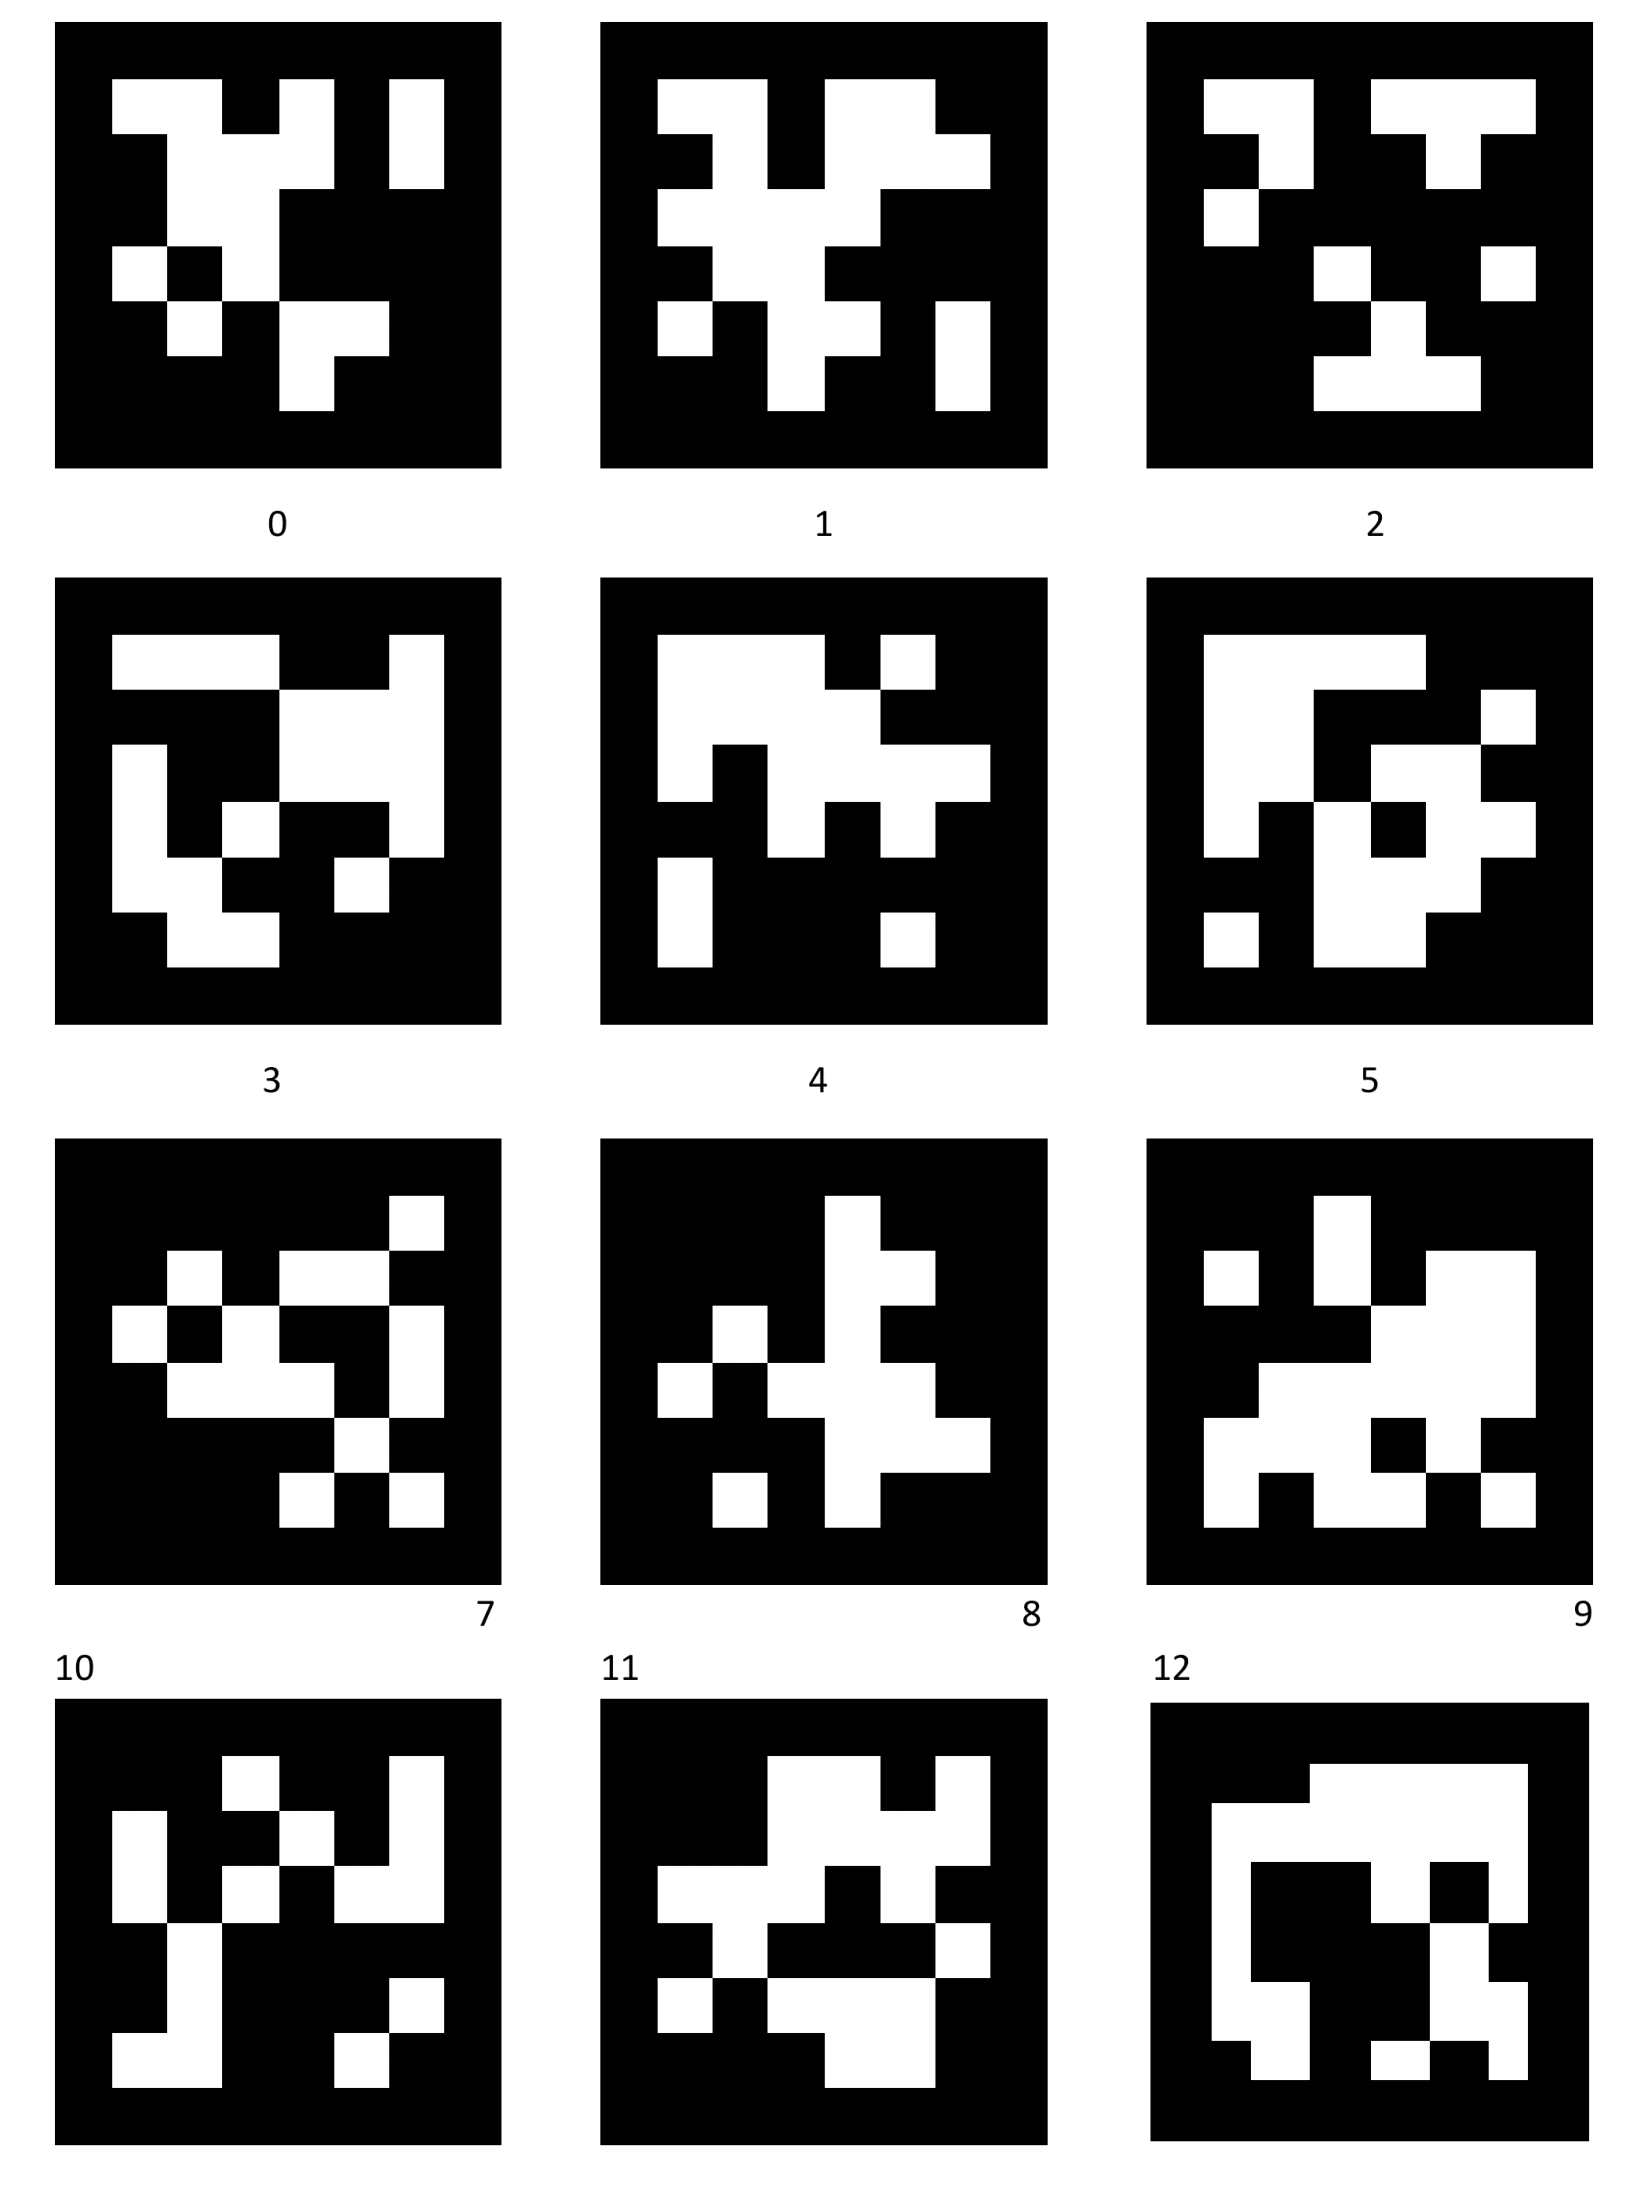
\includegraphics[width=.2\textwidth]{graphics/aptags.png}
    \caption{The calibration pattern using AprilTags \cite{Wang2016} that was used for the stereopair calibration.}
    \label{fig:aptags}
\end{figure}

Stereo pair calibration is a process of estimating the essential matrix $\mat{E}$ (defined in \autoref{sec:epipolar_geometry}) for a camera pair, which also expresses the relative rotation matrix $\mat{R}_{21}$ and relative translation vector $\vec{t}_{21}$ of a camera pair. 

There are multiple algorithms implementing a stereo pair calibration.
Usually, a calibration pattern is used as the one shown in \autoref{fig:chb} for a standard stereo camera with parallel or converging optical rays.
Most akgorithms assume that the whole pattern is seen in both images.
However, this is a disadvantage for cameras with a small overlapping zone and diverging optical rays.
For this reason, it is better to use some other pattern, for example, a set of apriltags \cite{Malyuta2019} which can be detected separately. 

\subsection{Least-square estimation of transformation}
\label{sec:lsq_umeyama}
The first approach assumes that an initial estimate of the relative pose of the cameras is obtained using a manual measurement, and that the only necessary step is to correct the pose of one camera with respect to the other.
Firstly it detects apriltag's from \textit{im1} and \textit{im2}, compute their 3D poses.
Then, estimate transformation parameters between two point sets, and find the correction transformation $\mat{T}_{correction}$.
The last step is to apply $\mat{T}_{correction}$ to $\mat{R}_{21}$ and $\vec{t}_{21}$ and obtain a corrected pose of the second camera.

\subsection{PnP-based estimation of transformation}
\begin{figure}[h]
    \centering
    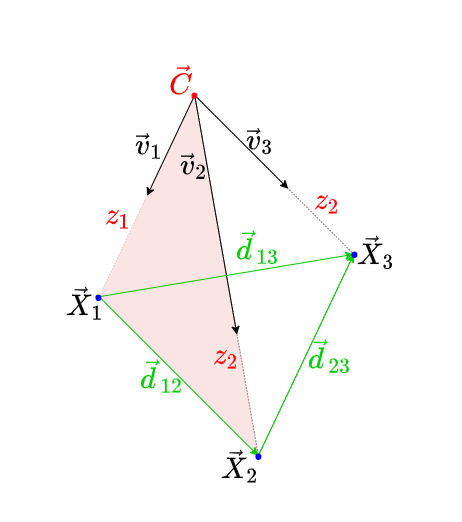
\includegraphics[width=.4\textwidth]{graphics/p3p.png}
    \caption[Visualization of the P3P problem.]{$\vec{C}$ is the camera center, vectors $\vec{v}_1$, $\vec{v}_2$ and $\vec{v}_3$ are unknown vectors with pointing to 3D points $\vec{X}_1$, $\vec{X}_2$ and $\vec{X}_3$ respectivly. The relative position of 3D points is known and expressed by vectors $\vec{d}_{12}$, $\vec{d}_{23}$ and $\vec{d}_{13}$. Scalars $z_1$, $z_2$ and $z_3$ are the absolute distances from each 3D point to the camera center in a world coordinate units (usually meters).}
    \label{fig:p3p}
\end{figure}

\label{sec:pnp}
Another, a more general approach is based on solving a Perspective-n-Point (PnP) problem.
PnP is the problem of estimating a camera pose (translation and rotation) given a known set of 3D points and theit respective 2D projections to an image of a calibrated camera.
Mathematically, the situation can be expressed as
\begin{equation}
    \label{eq:pnp_intro}
    \lambda_i \begin{bmatrix} \vec{m}_i \\ 1 \end{bmatrix} = \mat{K} \mat{R} (\vec{X}_i - \vec{C}), \;\; i = \{0..n\}.
\end{equation}
No initial pose estimation is needed for this algorithm, but it can accelerate the solver if there is one.

The situation when $n=3$ is the minimal amount of points to solve the PnP problem, this method is called P3P.  
Firstly, let us define a vector $\vec{v}_i \in \mathbb{R}^3$ corresponding to a projection of a point in the image $\vec{m}_i$ as $\vec{v}_i = \mat{K}^{-1}\begin{bmatrix}\vec{m}_i \\ 1 \end{bmatrix}$. From eq. \eqref{eq:pnp_intro}, the following relation can be obtained:
\begin{equation}
    \label{eq:p3p_gen}
    \lambda_i \vec{v}_i = \mat{R} (\vec{X}_i - \vec{C}).
\end{equation}
If there is no rotation, the situation will look like in \autoref{fig:p3p} where vectors $\vec{d}_i$ are known, so eq. \eqref{eq:p3p_gen} simplifies to a system of three equations with three unknowns (vector $\vec{C}$).
If there is a non-zero rotation, it can be elliminated first.
Let us define a helper variable $z_i$ as the distance of a point $\vec{X}_i$ from $\vec{C}_i$:
\begin{equation}
    \label{eq:p3p_rot}
    |\lambda_i| \cdot ||\vec{v}_i|| = || \vec{X}_i - \vec{C} || = z_i.
\end{equation}
Considering only angles between $\vec{v}_i$ and applying the cosine law per $\triangle{\vec{C}, \vec{X}_i, \vec{X}_j}$, for $i, j \in \{1, 2, 3\}, i \neq j$, the relation
\begin{equation}
    ||\vec{d}_{ij}|| = z_i^2 + z_j^2 - 2z_iz_jc_{ij}
\end{equation}
may be obtained, where $||\vec{d}_{ij}|| = || \vec{X}_j - \vec{X}_i ||$, $c_{ij} = \cos(\angle \vec{v}_i \vec{v}_j)$.
After solving the system of three equations with three unknown $z_i$, there will be up to 4 solutions.
Complex solutions, and other should be either verified on additional points \cite{Fischler1981} or sorted by reprojection error (refer \autoref{sec:error_reprojection}).
Having this, $\vec{C}$ can be found by trilateration (3 sphere intersection) from $\vec{X}_i$ and $z_i$; then $\lambda_i$ from \eqref{eq:p3p_rot} and $\mat{R}$ from \eqref{eq:p3p_gen}.

\section{Feature extraction, matching and filtering}
\label{sec:features}
In computer vision, \textit{features} typically refer to representations of unique pieces of information from the image scene, such as points, edges and objects.
A feature detector is an algorithm for extracting features from an image.
There are many such algorithms, but in this solution, the ORB features extractor is used. 
The authors in \cite{Rublee2011} claim that ORB has the same accuracy as the state-of-the-art SIFT detector while being a few times faster, which is also supported by other research \cite{Sharif2017}. 

Next step of the proposed method is mutually assosiating features in images from the two cameras, corresponding to the same physical objects in the environment. 
This is done by a feature matcher, which compares descriptors of the features provided by the feature detection algorithm.
Some feature extraction algorithms perform a brute-force comparison of all combinations of features, others use nearest neighbors approximations or even neural networks \cite{Sarlin2020}.

A brute-force matcher is one of the simplest matchers.
It takes one descriptor from one set, computes its similarity to all descriptors from the second set, and matches it with the most similar feature. 
This process is repeated to maximize the total overall similarity between two matched features.

Even after this process, there will be some outliers.
Distance from features to the corresponding epipolar lines can be used to filter them. 
This distance can be computed using the equation \autoref{eq:epiconstr}.
Its result is $0$ only in an ideal case; otherwise, the equation result will be the distance from the reprojected point to its corresponding epipolar line.

\section{Features position estimation}
Positions of the observed 3D points in the scene can be computed by having pairs of correspondent points taken by calibrated cameras.
This process is called triangulation.
Correspondences for triangulation are received as a result of features detection, matching and filtering.

\subsection{Shortest distance triangulation}
\label{sec:shortest_distance}
One triangulation method is based on finding the shortest distance between two rays.
According to the epipolar geometry properties described in \autoref{sec:epipolar_geometry} and visualized in \autoref{fig:epipolar_std}, vectors $\vec{d}_1$ and $\vec{d}_2$ intersects at the 3D point $\vec{X}$.
However, in the real world, the rays can be at some distance from each other due to imperfect stereo pair calibration, so $\vec{X}$ is the point closest to both lines.

It is possible to compute $\vec{d}_1$ and $\vec{d}_2$ in a common coordinate frame from $\vec{m}_1$ and $\vec{m}_2$, since the relative pose of the cameras is known.
Then, let us define two lines $d_1$ and $d_2$ in a vector form:
\begin{equation}
    \label{eq:shortest_d1}
    d_1: p_1 = \vec{C}_1 + t \vec{d}_1,
\end{equation}
\begin{equation}
    \label{eq:shortest_d2}
    d_2: p_2 = \vec{C}_2 + s \vec{d}_2,
\end{equation}
where $\vec{d}_1$ and $\vec{d}_2$ are directional vectors, $\vec{C}_1$ and $\vec{C}_2$ are 3D points located on the respective lines (camera centers in this case), $s \in \mathbb{R}^{3}$ and $t \in \mathbb{R}^3$ are free parameters that uniquely define points $p_1$ and $p_2$. 
Distance between the two lines is minimal at the point where the vector $\vec{l} = p_2 - p_1$ is orthogonal to $d_1$ and $d_2$, which can be expressed using a dot product as 
\begin{equation}
    \label{eq:ldd1}
    \vec{l} \cdot \vec{d}_1 = 0,
\end{equation}
\begin{equation}
    \label{eq:ldd2}
    \vec{l} \cdot \vec{d}_2 = 0.
\end{equation}
After substituting eqs. \eqref{eq:shortest_d1} and \eqref{eq:shortest_d2} to these equations, a system of two equations with two unknowns $s$ and $t$ is obtained.
This system has a unique solution unless the rays are parallel.
Using $s$ and $t$, the points $\vec{p}_1$ and $\vec{p}_2$ can be obtained and then $\vec{X}$ is calculated as $\vec{X} = \frac{p_1 + p_2}{2}$.

\subsection{SVD Triangulation}
\label{sec:svdtriang}
Triangulation using Singular Value Decomposition (SVD) is another method that is more robust and more widely used.
It computes 3D points from 2D correspondences using the camera matrices $\mat{P}_1$, $\mat{P}_2$. 
This method is proved and described in detail in \cite{hartley_zisserman_2004}, p.312. Here, a short summary is provided.

The projection equation \eqref{eq:projection} can be rewritten as
\begin{equation}
    \lambda_i \begin{bmatrix} 
        u_i \\ v_i \\ 1 \end{bmatrix} = \mat{P}_i
    \begin{bmatrix} \vec{X} \\ 1
    \end{bmatrix},
\end{equation} 
where $\mat{P}_i$ decomposes as in eq. \eqref{eq:p_general}, and $\lambda_i \neq 0$, $i \in \{1, 2\}$.
After eliminating $\lambda_1$, $\lambda_2$ we obtain the following set of equations:
\begin{equation}
    \mat{D} \begin{bmatrix} \vec{X} \\ 1 \end{bmatrix} = \vec{0}, \;\;\;\;\;
    \mat{D} = \begin{bmatrix}
        u_1 (\vec{p}_{1, 3})^\top - (\vec{p}_{1, 1})^\top \\
        v_1 (\vec{p}_{1, 3})^\top - (\vec{p}_{1, 2})^\top \\
        u_2 (\vec{p}_{2, 3})^\top - (\vec{p}_{2, 1})^\top \\
        v_2 (\vec{p}_{2, 3})^\top - (\vec{p}_{2, 2})^\top \\
    \end{bmatrix}, \;\;\;\;\; \mat{D} \in \mathbb{R}^{4 \times 4}.
\end{equation}


SVD decomposition of $\mat{D}^T\mat{D}$, which is a solution of the equation

\begin{equation}
    \mat{U}\mat{S}\mat{V}^\top = \mathsf{SVD}(\mat{D}^\top\mat{D}),
\end{equation}

where $\mat{U}$ and $\mat{V}$ are orthogonal matrices and $\mat{S}$ is a non-negative diagonal matrix.

The solution of the triangulation would be the eigenvector corresponding to the smallest eigenvalue, the last columt of the matrix $\mat{U}$, where $\vec{u}_4 = (u_1', v_1', u_2', v_2')^\top$.

% The solution is $u_4$, the last column of the $\mat{U}$ matrix from $\mathsf{SVD}(\mat{D}^\top \mat{D}) = \mat{U}, \mat{S}, \mat{V}^\top$.




\clearpage
\chapter{Implementation}
\label{chapter:implementation}

This chapter describes the implementation of the solution.
The used hardware is presented in \autoref{sec:impl_hardware}, the software tools and integration of all parts together in \autoref{sec:impl_software}. The code can be found on GitHub: stereo pair driver\footnote{\url{https://github.com/Myralllka/UAV_basler_stereopair_driver}} and the main module\footnote{\url{https://github.com/Myralllka/UAV_localisation_from_cameras}}.

\section{Hardware}
\label{sec:impl_hardware}
\begin{figure}[ht]
  \begin{subfigure}[b]{0.49\textwidth}
    \centering
    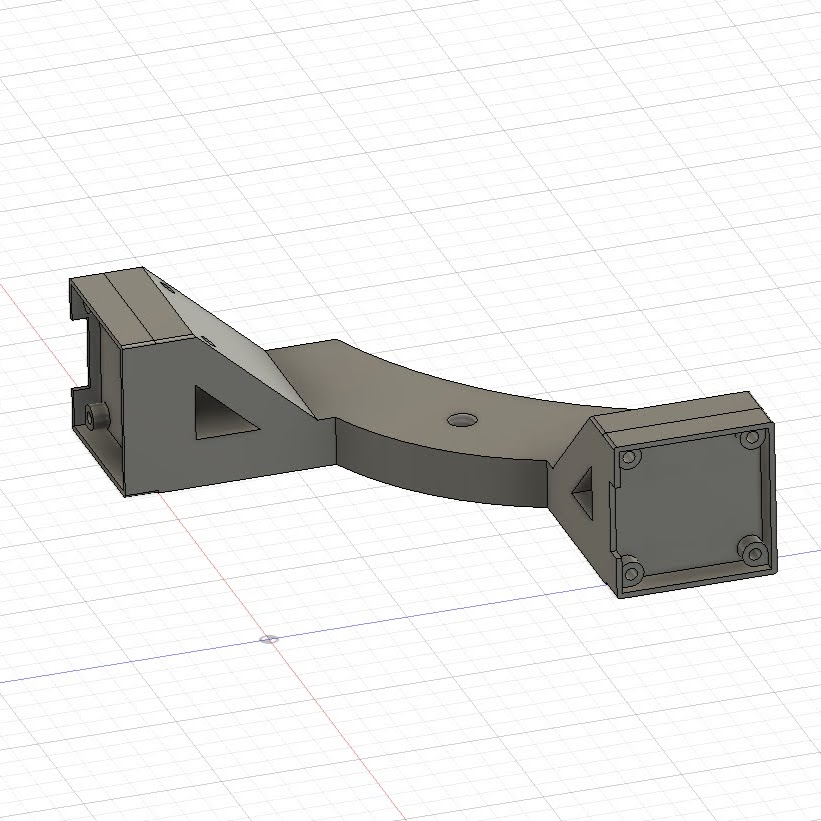
\includegraphics[width=\textwidth]{graphics/CAD.jpg}
    \caption{The CAD model of the prototype.}
    \label{fig:proto_scheme}
  \end{subfigure}
  \hfill
  \begin{subfigure}[b]{0.49\textwidth}
    \centering
    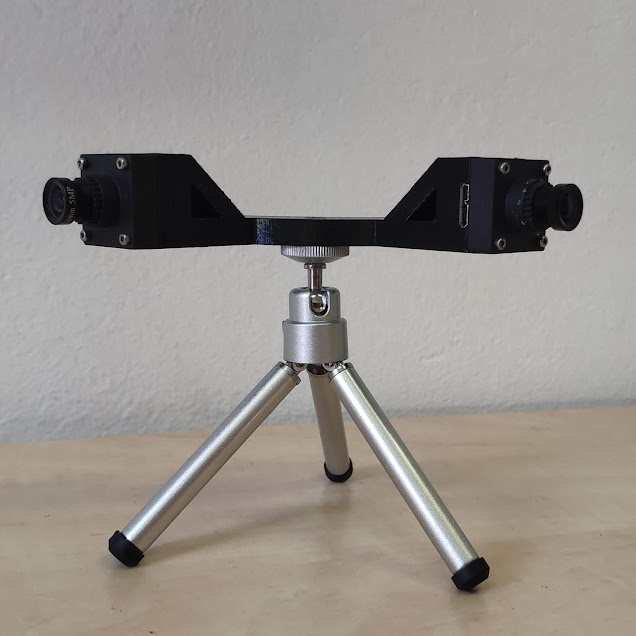
\includegraphics[width=\textwidth]{graphics/prototype.jpg}
    \caption{The printed prototype}
    \label{fig:proto_printed}
  \end{subfigure}
  \caption{A prototype of the proposed solution.}
  \label{fig:prototype}
\end{figure}

CAD model of a camera mount was created in the Fusion360 software considering the requirements of a $90^\circ$ rotation between cameras and distance of the cameras close to the average MAV size.
A picture of the design from the CAD software is in \autoref{fig:proto_scheme}.
The 3D-printed prototype with the cameras mounted is in \autoref{fig:proto_printed}

Basler daA1600-60um cameras were chosen for this project because they have a global shutter which is important when deployed onboard a fast-moving platform, good image quality and high framerate, making them suitable for the proposed method based on the assumptions defined in \autoref{sec:problem_definition}. 
More details regarding camera parameters are in \autoref{tab:daA1600}.

\begin{table}
    \begin{center}
      \begin{tabular}{ l l }
      \hline
      Parameter              & Value             \\ \hline
      Lens mount type        & S-mount           \\
      Data transfer protocol & USB 3.0           \\
      Max. frame rate        & 60 fps            \\
      Resolution (HxV)       & 1600 px x 1200 px \\
      Resolution             & 2 MP              \\
      Price                  & 289.00 EUR        \\ \hline
      \end{tabular}
    \end{center}
    \caption{daA1600-60um specifications.}
    \label{tab:daA1600}
\end{table}

Lenses of the cameras were chosen so that the resulting horizontal FOV is approximately $120^\circ$, which provides a sufficient overlapping zone to detect features in $\Psi$ (see \autoref{fig:sch_stereo}).

The solution was developed and tested on the Lenovo ThinkPad X280 with Intel(R) Core i7-8550U CPU and 16Gb RAM.
Intel NUC with Intel(R) Core i7-10710U CPU and 16Gb RAM is used as the onboard computer for the MAV.
No dedicated GPU is needed.

\section{Software tools}
\label{sec:impl_software}

The proposed solution uses the Robot operating system (ROS) \cite{Rospaper} as a middleware.
ROS is an open-source ecosystem with hundreds of already implemented algorithms and libraries to interact between different parts of a robot's system, such as sensor drivers, image processing algorithms, planners, controllers etc.
The AprilTag detector and a driver for Basler cameras used in this thesis are based on publicly available modules from the ROS community.

The MRS UAV system \cite{Baca2021} is used as a drone control environment. It is based on ROS, but it is a unique framework for MAVs to implement and test path planning, control, computer vision, object tracking, and many more MAV-related problems.

The OpenCV\footnote{\url{https://opencv.org/}} open-source computer vision library and the Eigen\footnote{\url{http://eigen.tuxfamily.org}} open-source library for efficient linear algebra were used for the implementation.
All of the software presented in this thesis was implemented in C++.

\begin{figure}[ht]
    \centering
    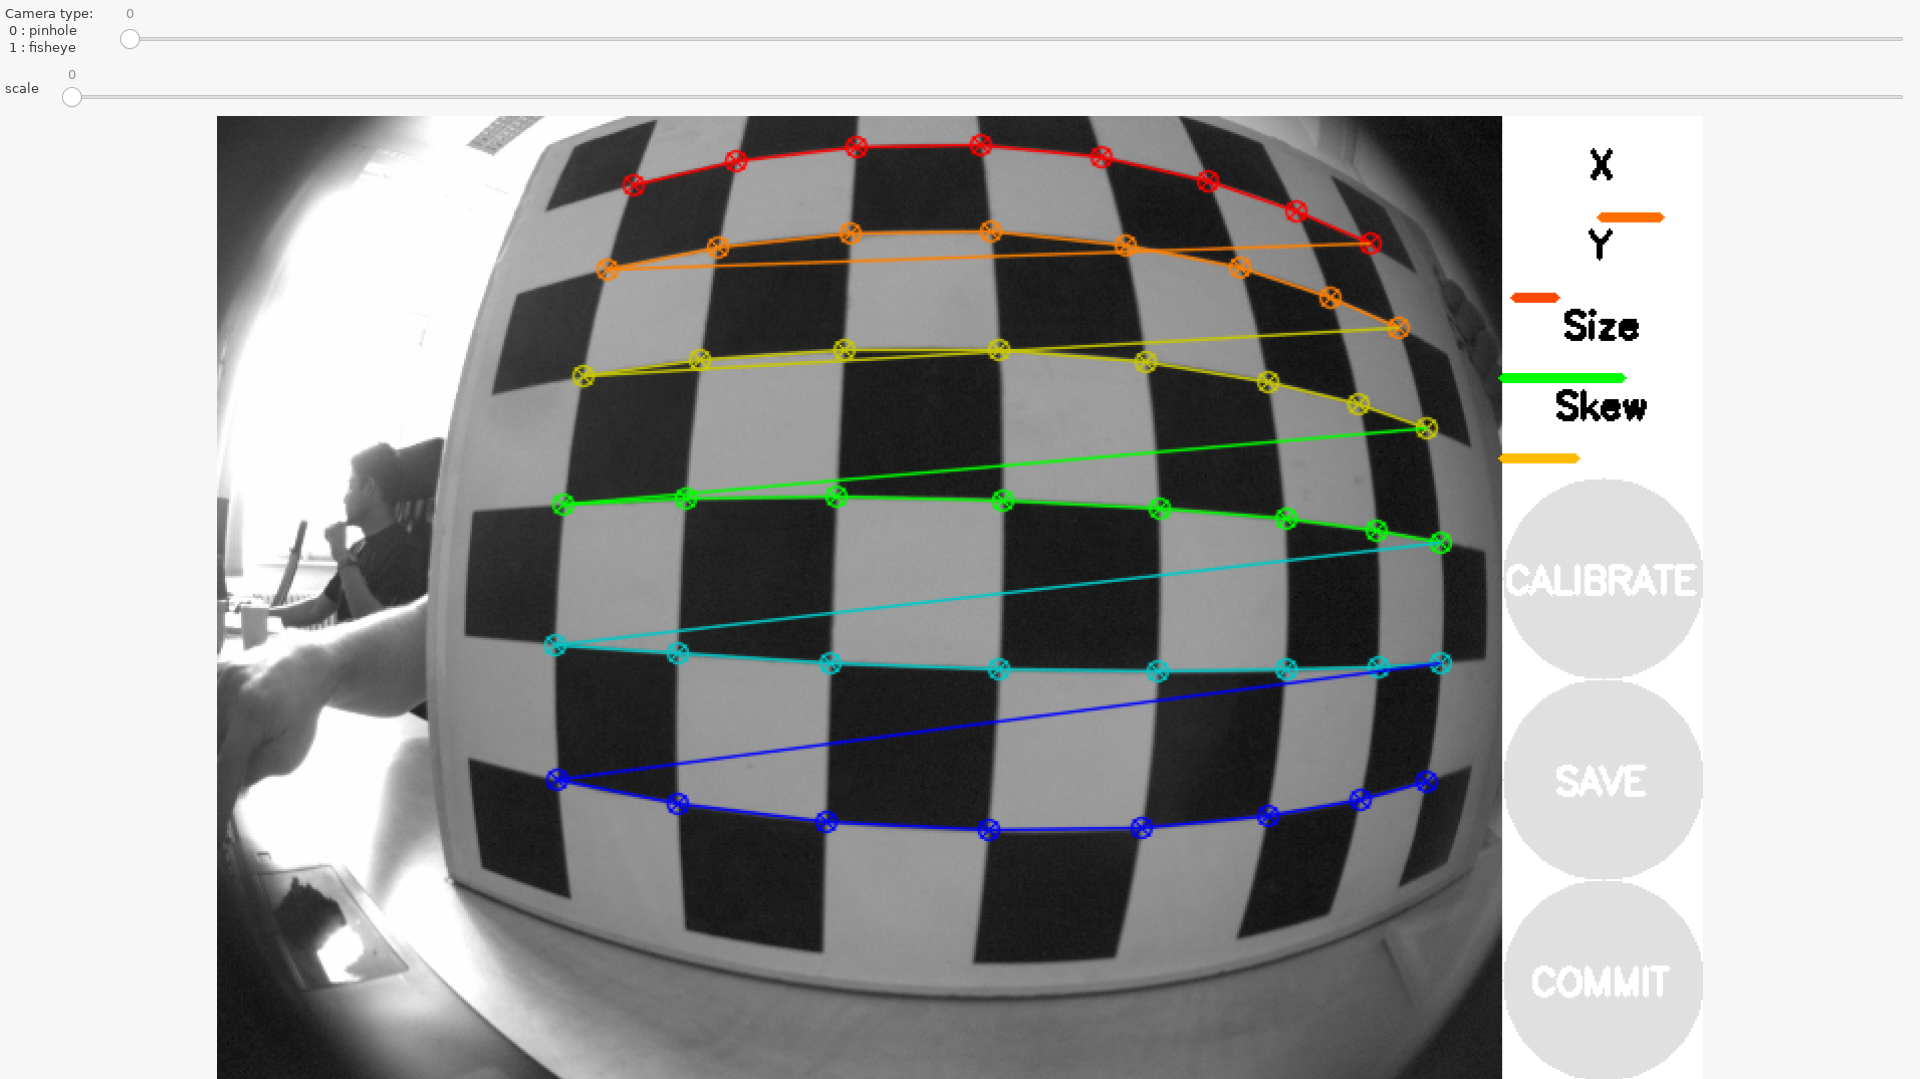
\includegraphics[width=.6\textwidth]{graphics/calibration.png}
    \caption{The single camera calibration process.}
    \label{fig:calib}
\end{figure}

Calibration of parameters od the camera projection and distortion models (described in \autoref{sec:meth_calib}) was performed using the ROS Camera Calibration package\footnote{\url{http://wiki.ros.org/camera_calibration}}.
A chessboard pattern is used for the calibration, and its physical parameters must be specified to the calibration program.
The calibration process itself is done interactively using a graphical user interface (shown in \autoref{fig:calib}).
The interface displays the progress of the process to the user, and when a sufficient dataset is obtained, the user can trigger the parameter optimization. 
Results of the optimization are then saved to a file for later use.

\begin{figure}[ht]
    \centering
    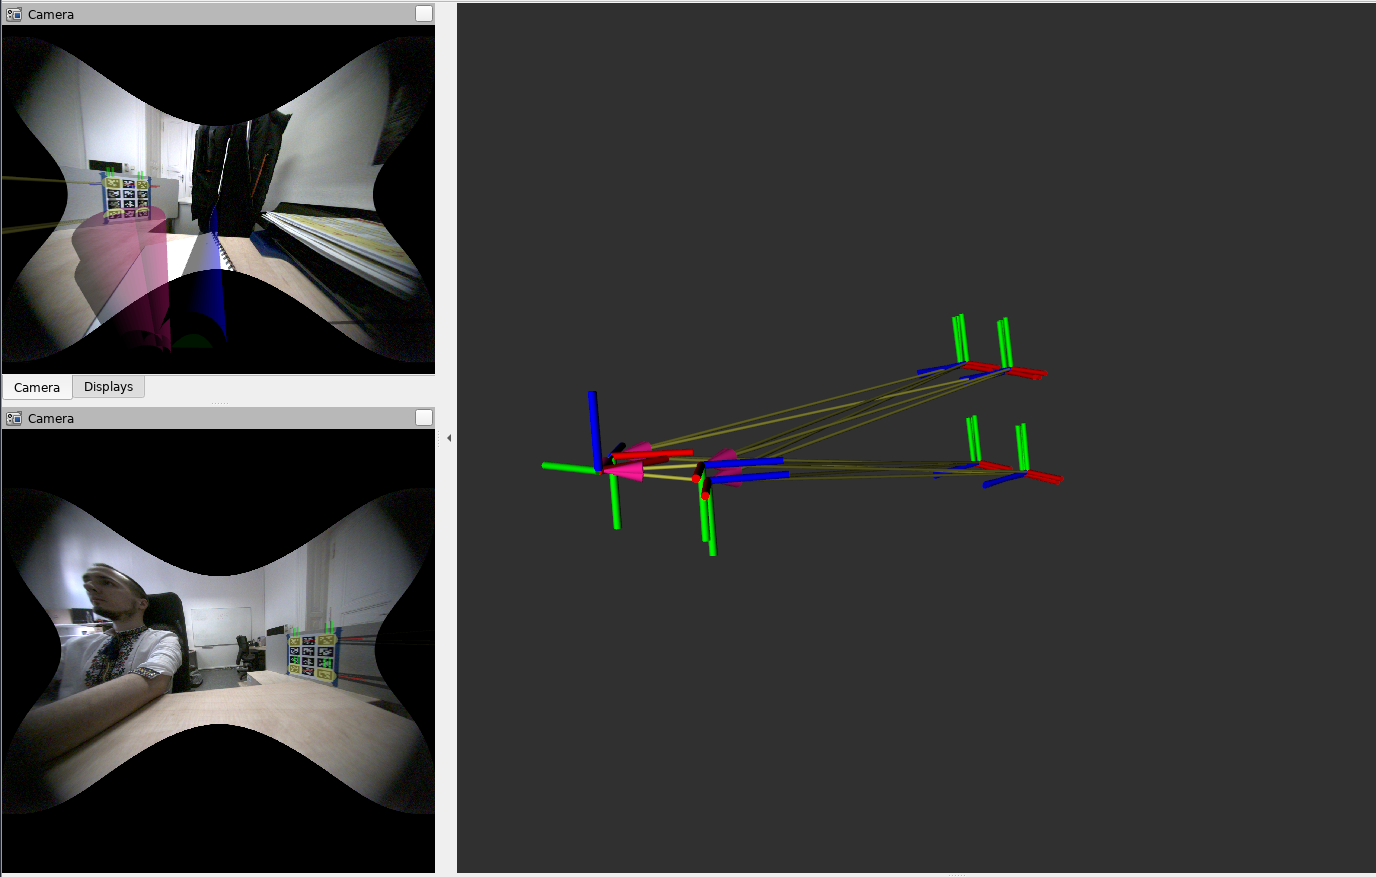
\includegraphics[width=.8\textwidth]{graphics/calib_process.png}
    \caption[The stereocamera calibration process]{The stereo pair calibration. In the left side there are views from the right camera (top) and left camera (bottom). Both cameras observing the AprilTag's pattern. On the right side there is a visualization from the ROS Vizualisation tool (rviz) of initial poses of both cameras, AprilTags and the corrected right camera pose.}
    \label{fig:calib_stereo}
\end{figure}

The two calibration methods described in \autoref{sec:stereocalib} were both implemented to use an AprilTag calibration pattern, shown in \autoref{fig:aptags}.
The main reason why this pattern was chosen is that each tag can be detected individually, so there is no need to have all of them simultaneously in the overlapping zone.
The first method, described in \autoref{sec:lsq_umeyama}, is implemented using the "Least-square estimation of transformation between two point sets" \cite{Umeyama1991} implementation from Eigen.
Measurements from the CAD model of the camera mount were used as the initial estimate of the cameras' relative pose.
The second method, described in \autoref{sec:pnp}, is implemented using the OpenCV PnP solver.
Because the publicly available implementation of the AprilTag detector outputs only 3D poses of detected tags, the detector was modified to output also 2D coordinates of corners of the detected markers, which is needed for the PnP algorithm and during the debug session for computing the reprojection error.
The calibration process is in the \autoref{fig:calib_stereo}.

\begin{figure}[ht]
  \centering
  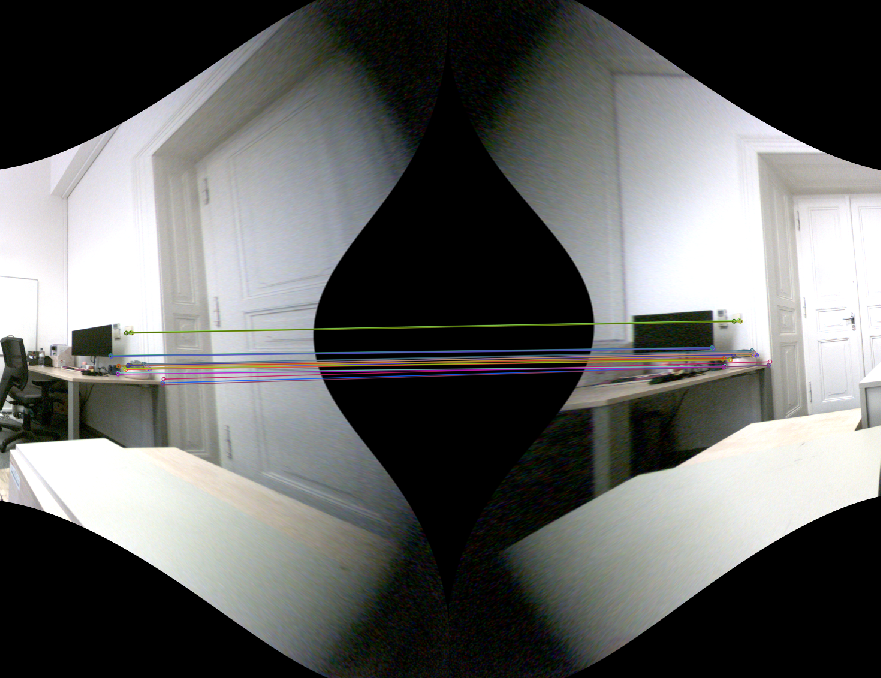
\includegraphics[width=0.92\textwidth]{graphics/corresp.png}
  \caption[The result of features detection, matching and outliers filtering.]{In the image ...} :TODO
  \label{fig:corresp_life}
\end{figure}
\begin{figure}[ht]
  \centering
  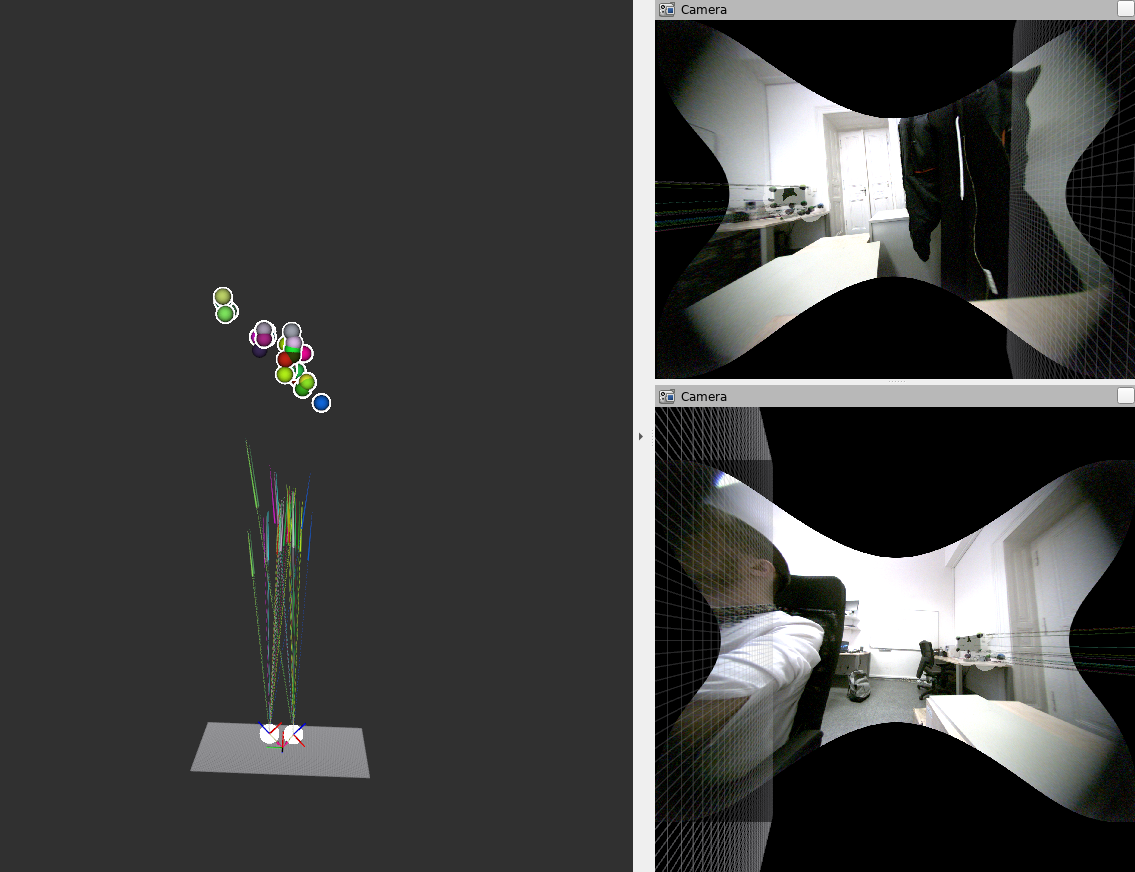
\includegraphics[width=0.49\textwidth]{graphics/res_trangulation.png}
  \caption{Triangulated points}
  \label{fig:triang_life}
\end{figure}

After both cameras and the stereo pair are calibrated, the following steps are feature detection, matching and filtering, described in \autoref{sec:features}.
The example from a real-world experiment is in \autoref{fig:corresp_life}.

The synchronization is done on a stereo pair driver level.
As described in \autoref{sec:features}, the ORB detector and a brute-force matcher implementation from the OpenCV were used for feature detection and matching.
The next step is reconstructing the 3D scene from the obtained feature pairs.
The method described in \autoref{sec:shortest_distance} is implemented from scratch, and the implementation of triangulation described in \autoref{sec:svdtriang} is taken from OpenCV.
In the \autoref{fig:triang_life} in the left part there are triangulated points shown as colored spheres, and rays pointing from camera centers to feature points colored with the same color as corresponding feature.
In the right side there are cameras' views.


% As a result, obstacles in the cameras' overlapping zone are detected in a format of the point cloud and correspondent feature points on both images.
% Recalling the \autoref{fig:intro_general}, the proposed solution providing a pointcloud with obstacles in a red zone at each timestamp $t_i$. 

\clearpage
\chapter{Evaluation}
\label{chapter:evaluation}

\section{Calibration quality}
Another tool from the same ROS Camera Calibration package is used to compute the camera calibration error.
It continuously outputs a reprojection $\mathsf{RMS}$ (Root Mean Squared), which is defined as
\begin{equation}
    \mathsf{RMS}(x) = \sqrt{\frac{\sum_{i=1}^{N}{(x_i - \hat{x}_i)^2}}{N}}
\end{equation}
where $x$ is one measured data sample from the experiment, $\hat{x}$ is a ground-truth data, and $N$ is a sample size.
After launching this tool, we were moving a pattern in front of each camera to collect some data and analyse it.
The reprojection error varies depending on the pose of the chessboard but, in general, is quite stable, see \autoref{tab:camcalib_eval}.

\begin{table}[ht]
    \begin{center}
      \begin{tabular}{ ll l l }
      \hline
      && Left camera & Right camera \\ \hline
      mean of RMS reprojection error & [px] & 0.06323214286 & 0.05357391304 \\
      variance of RMS reprojection error & [px] & 0.00001159968 & 0.00002222914 \\
      \end{tabular}
    \end{center}
    \caption{RMS reprojection error of the ROS Camera Calibration results.}
    \label{tab:camcalib_eval}
\end{table}

\section{Triangulation quality}
Two experiments were concluded to measure the triangulation quality.
The same pattern with visible key points in a featureless environment was used \autoref{fig:exp_process}.

\subsection{Experiment setup}
\label{sec:eval_setup}

\begin{figure}[ht]
    \centering
    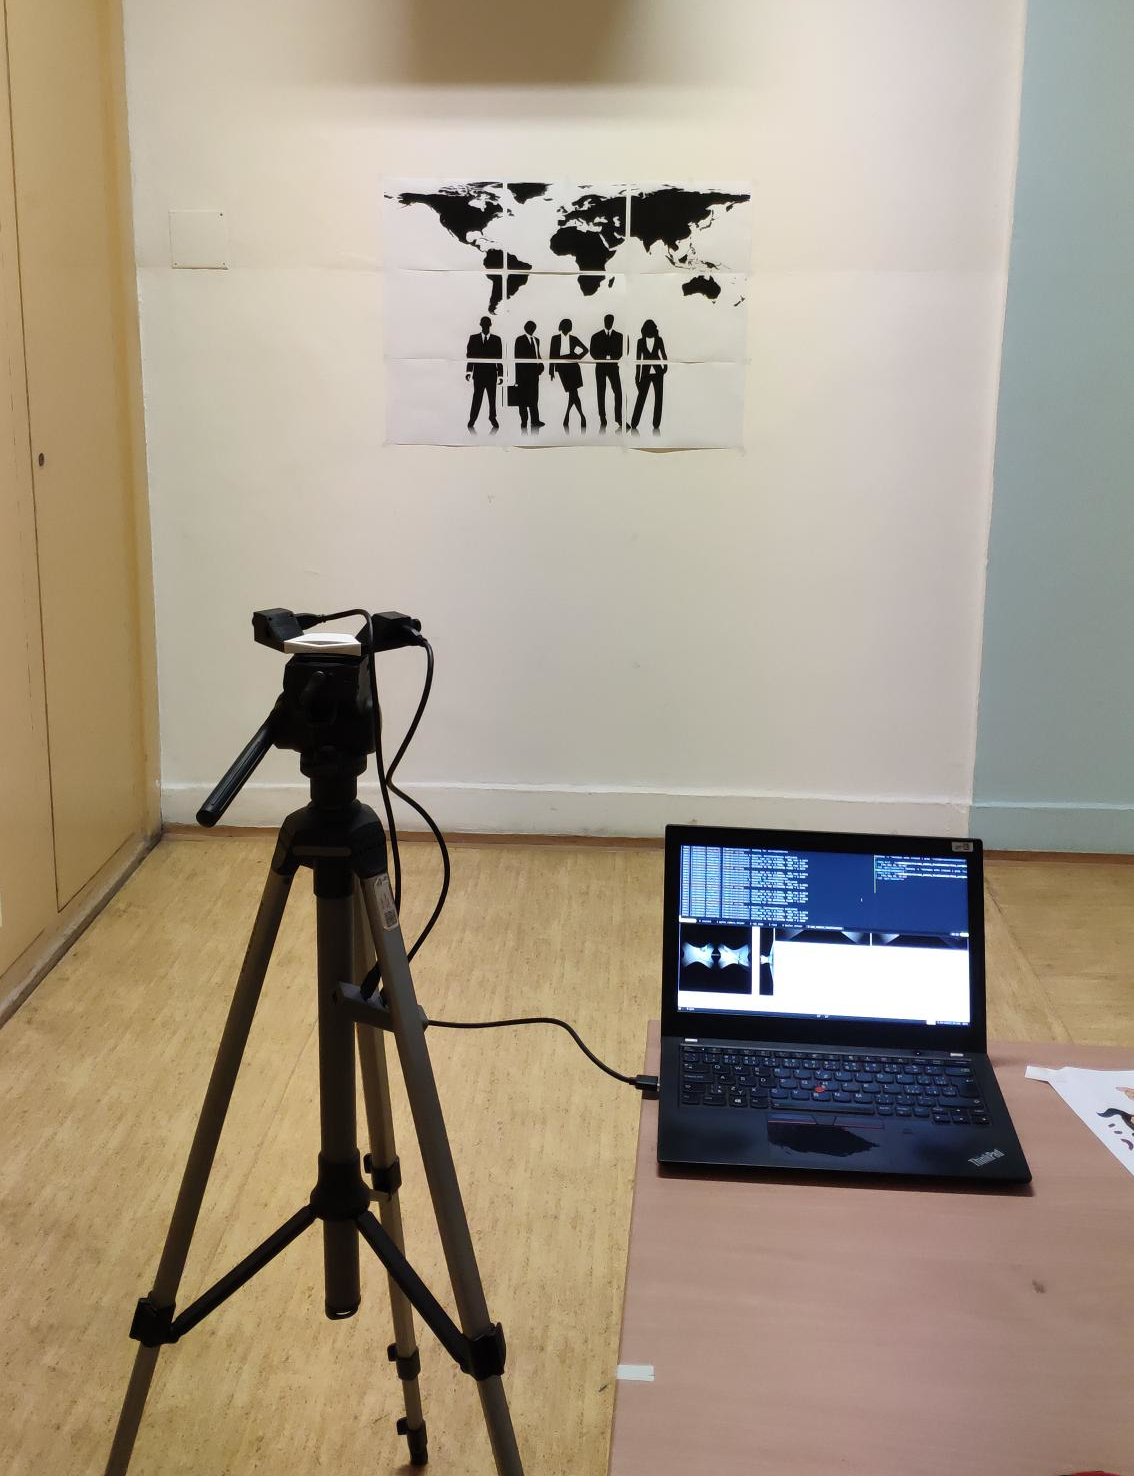
\includegraphics[width=0.6\textwidth]{graphics/experiment_setup.png}
    \caption[The setup for experiments]{The setup for experiments. 
    The designed prototype is located on a tripod, at distance $d$ from the plane $\Omega$ with visual features.
    The with y-z plane of the cameras' common coordinate frame is parallel with $\Omega$. 
    A set of 9 A4 papers with features was used to make $\Omega$ distinguishable.}
    \label{fig:exp_process}
\end{figure}

\begin{figure}[ht]
  \centering
  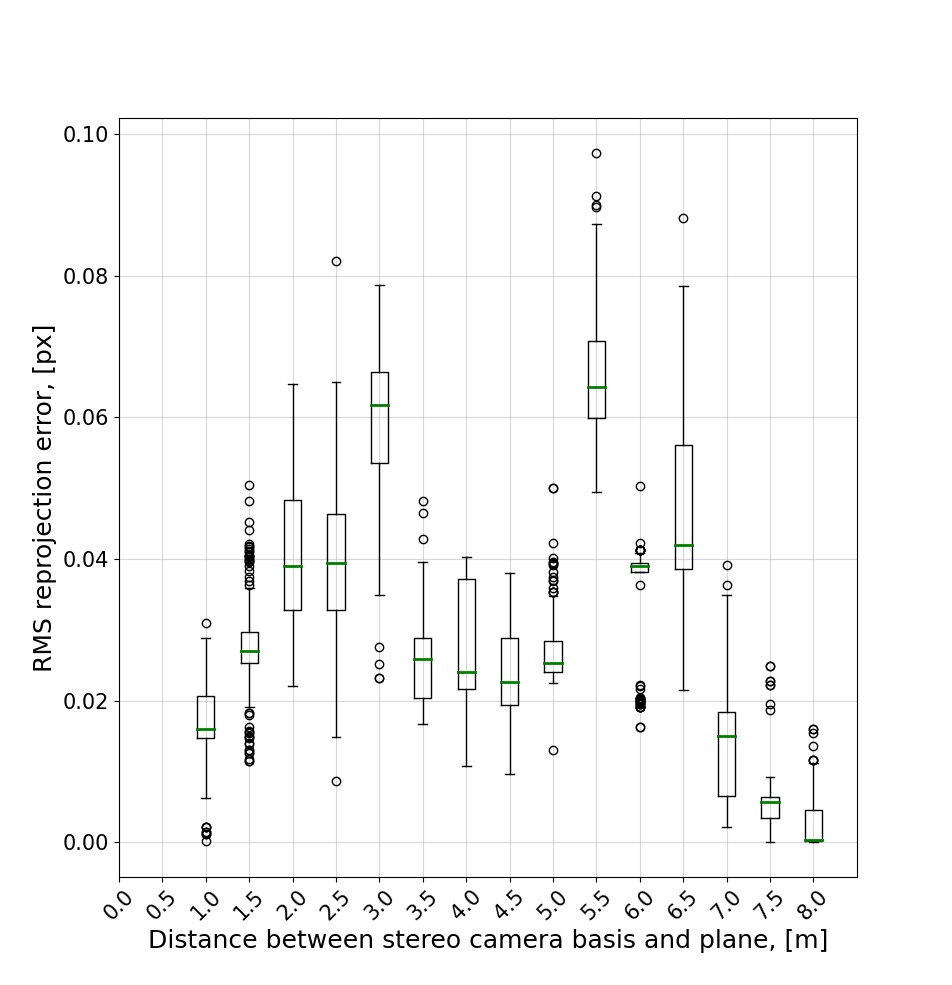
\includegraphics[width=0.5\textwidth]{graphics/experiment_1_repro_error.png}
  \caption[Stereo pair setup RMS reprojection error.]{Stereo pair setup RMS reprojection error. 
  Green lines represents the median for each $n$ measurements at a distance $d$. 
  Box is drown from the first quartile to the third quartile.
  The whiskers go from each quartile to the minimum and maximum.
  Black points represents outliers.
  }
  \label{fig:exp_1_repro}
\end{figure}

\begin{figure}[ht]
  \begin{subfigure}[ht]{0.49\textwidth}
    \centering
    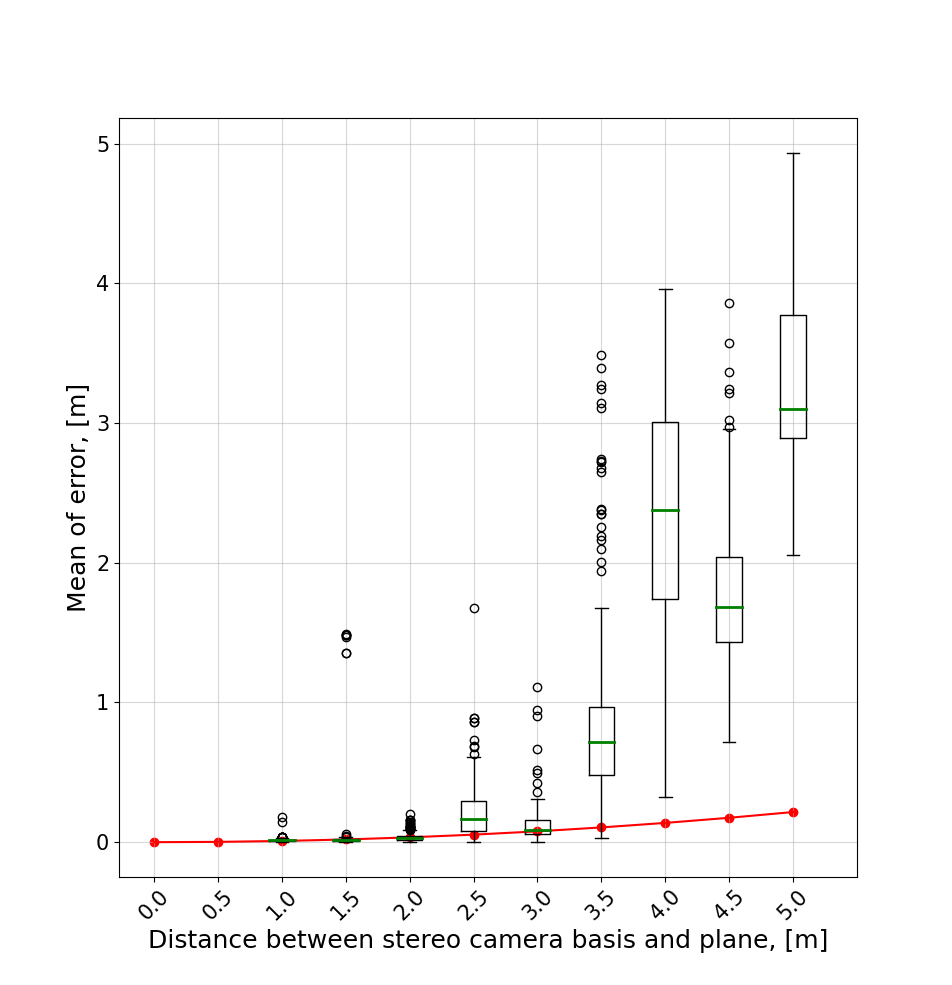
\includegraphics[width=\textwidth]{graphics/experiment_1_general.png}
    \caption[The first experiment results.]{The first experiment results. Red line represents the theoretical error for the given setup. Green lines represents the median for each $n$ measurements at a distance $d$ from the stereo camera to $\Omega$.
    Box is drown from the first quartile to the third quartile.
    The whiskers go from each quartile to maximum and minimum.
    Black points represents outliers.}
    \label{fig:exp_1_chart_dists}
  \end{subfigure}
  \hfill
  \begin{subfigure}[ht]{0.49\textwidth}
    \centering
    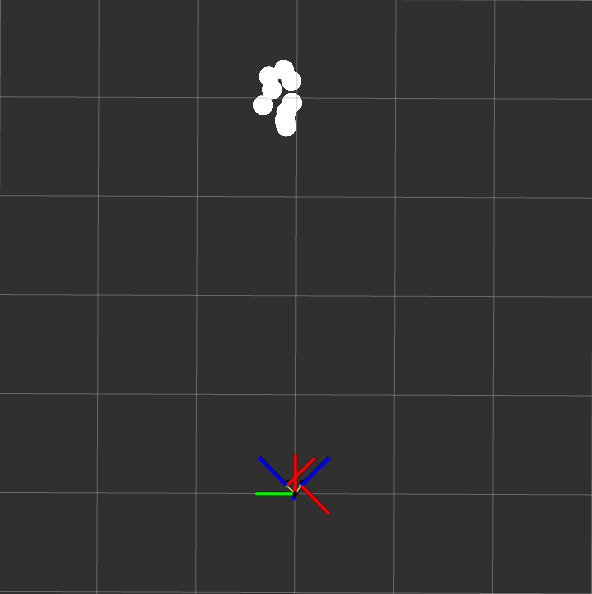
\includegraphics[width=\textwidth]{graphics/experiment_1_4m.png}
    \caption[Top view of the experiment.]{Top view of the experiment. 
    The grid's cell size is $1$m$\times$$1$m.
    The colored axes represent the stereo pair's coordinate system.
    Red color stands for $X$ axis, green for $Y$ and blue for $Z$.
    The basis aligned with the grid represents the stereo camera basis, $X$ axis towords the point cloud.
    The point cloud (white dots) represents the 3D points reconstructed from feature points seen by both cameras.}
    \label{fig:exp_1_topview}
  \end{subfigure}
  \caption{Results from the first experiment: distance to the estimated plane.}
  \label{fig:exp_1_exp}
\end{figure}

\begin{figure}[ht]
    \centering
    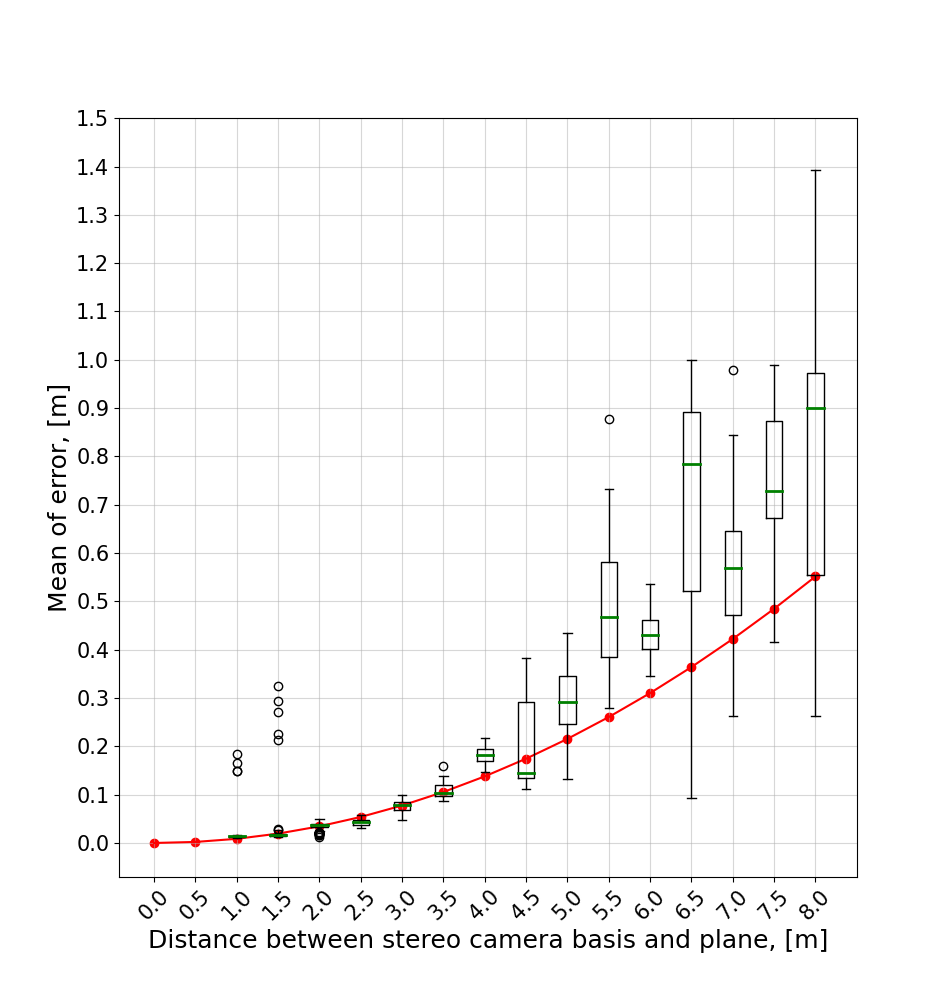
\includegraphics[width=\textwidth]{graphics/experiment_2_general.png}
  \caption[The second experiment results.]{The second experiment results. Red line represents the theoretical error for the given setup.
  Green lines represents the median for each $n$ measurements at a distance $d$. Box is drown from the first quartile to the third quartile.
  The whiskers go from each quartile to the minimum and maximum.
  Black points represents outliers.}
  \label{fig:exp_2_general}
\end{figure}

The reprojection error is not a good metric to evaluate the triangulation performance because, with the distance increasing, the feature points are closer together, and the reprojection error decreases (see \autoref{fig:exp_1_repro}).
To measure the quality of distance estimation, a different approach was chosen.
A pattern with multiple features was attached to a white wall in a corridor within a featureless environment.
The camera prototype on a tripod was located at a fixed distance from the wall and was set up so that its $y-z$ plane was parallel to the wall as in \autoref{fig:exp_process}.
Based on this, we assume that the ground-truth position of all observed 3D points lies on a plane whose orientation and distance from the coordinate frame's origin are known.

Let us define the wall plane as $\Omega$, the distance from the origin of the stereo pair's common frame to the wall as $d$, an estimated plane as $\Omega'$ and an estimated distance to the plane as $d'$.
The number of timestamps for each experiment is $n$, and $i$ is a timestamp index, $i \in \{1 \dots n\}$.

The ground-truth distance was measured with the measuring tape, and the tripod was placed at a distance $d$ from the wall. 
Then $n$ measurements were made, and obtained data were collected and saved to post-process them separately, analyse and obtain plots.

The main goal of experiments is to measure the precision of triangulation and compare it with the theoretical error, introduced in \cite{cv_theoretical_error} as a function of the distance based on the geometrical and optical parameters of the setup.
The theoretical error is defined as
\begin{equation}
    e_Z = \frac{Z^2 \delta}{bf},
\end{equation}
where $Z$ is the real distance in, $\delta$ is a disparity error (error for keypoints matching, here - maximum possible distance to the corresponding epipolar error is used), $f$ is a focal length and $b = \lVert \vec{b} \rVert$ (see \autoref{fig:sch_stereo}).
To compute the theoretical error for the current prototype, the following data was used: $\delta=1$px, $f=38$mm and $b=14.5$mm.

\subsection{Distance to an estimated plane}
\label{sec:exp1}
For each set of 3D points corresponding to a specific distance $d$, the plane $\Omega'$ is estimated using RANSAC to filter outliers (an implementation from PCL was used).
The error is defined as
\begin{equation}
    e_i = \frac{1}{k}\sum_{j=0}^{k}{|d - d'_i|},
\end{equation}
where $d'_i$ is a distance to $\Omega'$ for each measurement.

The absolute error $e_i$ for distance of $d$ for this experiment was from $1$m to $5$m with a step of $0.5$m.
The result of this experiment is shown in \autoref{fig:exp_1_chart_dists}.
According to the figure, the distance deviates significantly after $3.5$m, and the error grows much faster than estimated.
In \autoref{fig:exp_1_topview} the topview of the experiment is shown for $d=4$m.
It can be seen that the plane can not be estimated correctly at this distance using RANSAC anymore because of a small error for each triangulated point.

\subsection{Distance to a predefined plane}
\label{sec:exp2}
With increasing the distance $d$, feature points become less distinguishable due to the limited resolution of the camera.
In \autoref{fig:exp_process}, the estimated plane $\Omega$ is inaccurate from a certain distance because of high noise in the $X$ direction of the points and low spread of the points in the $Y-Z$ direction (see \autoref{fig:exp_1_topview}), but still, the points are close to the actual plane $\Omega$.
That is why the second experiment was constructed.

The experiment was done using the same setup as described in \autoref{sec:eval_setup}. 
The difference is that $\Omega'$ is not estimated using the least squares RANSAC method to fit the plane to the points, but as the plane parallel to $\Omega$ on a distance $e'_i$, that is defined as
\begin{equation}    
    e'_i = \frac{1}{k} \sum_{j=0}^{k}{|p'_j|},
\end{equation}
where $k$ is the number of keypoints detected at a timestamp $t_i$, and $p'_j$ is the distance from point $\vec{p}'_j$ to $\Omega$.

% In \autoref{fig:exp_2_general} the red line represents the theoretical error for the proposed setup.

The ground-truth distance $d$ for the current experiment was from $1$m to $8$m as the maximum distance at which key points can be detected (empirically found) with a $0.5$m step.
The result of the second experiment is shown in \autoref{fig:exp_2_general}, where the received data follows the theoretical up to $4.0$ meters with a small deviation. 
After that, it also follows the pattern but with a bigger variance.
One possible problem here is that the theoretical error does not include the error from the feature detector and matcher.
The second one is that there is an error in camera calibration and fixed focal length (cameras were calibrated on a small distance up to $3$m), so detected patterns on bigger distances are blurred and less detectable. 

\section{Rate testing}
To ensure that obstacles can be detected, not only triangulation quality is important, but also the rate at which the MAV can receive the data from the obstacle avoidance module and the delay of the data.
The data rate, maximal and minimal delays for 5min are shown in \autoref{tab:eval_freq}.
\begin{table}[ht]
    \begin{center}
      \begin{tabular}{ll}
      \hline
        Parameter & Value \\
        Minimal delay &  0.042s \\
        Maximal delay &  0.196s \\
        Average rate & 10.607Hz \\ 
      \end{tabular}
    \end{center}
    \caption{Measured data delay and rate of the proposed system.}
    \label{tab:eval_freq}
\end{table}
 
\section{Experiments summary}
The quality of the distance estimation to obstacles was demonstrated in the two experiments.
The first experiment, described in \autoref{sec:exp1}, shows that the precision of the proposed method is relatively high for distances up to 3m, and the second experiment, described in \autoref{sec:exp2} provided further insight into the statistics of the error over longer distances. 
The estimated distance error on $3$m is less than $3\%$.
The maximum distance at which 3D points could be reliably estimated is $8$m with an error of up to $1$m.
On further distances, feature points can not be reliably detected anymore due to the camera resolution and focal length (cameras were calibrated on distances up to $2$m).
The proposed solution works with an average frequency of $10$Hz.

\clearpage
\chapter{Conclusion}
\label{chapter:conclusion}

% Here the proposed algorithm can help - it gives common points to an algorithm, so instead of SfM from 2 images it does SfM from 4 images but with bigger pressision, because $T_{static}$ remains the same, and the only necessary transformation that should be estimated is $T_{t_0t_1}$, and the innertial module can help with that.

% Another possible approach is to use already working SfM algorithm implementation for a left and rigth camera separately to obtaine two pointclouds, and then align them and fix a scale using Iterative closest point algorithm with respect to fixed red pointcloud
\clearpage

%\include{Chapters/Chapter3}
%\include{Chapters/Chapter4} 
%\include{Chapters/Chapter5} 

%----------------------------------------------------------------------------------------
%	THESIS CONTENT - APPENDICES
%----------------------------------------------------------------------------------------

\appendix % Cue to tell LaTeX that the following "chapters" are Appendices

% Include the appendices of the thesis as separate files from the Appendices folder
% Uncomment the lines as you write the Appendices

% \include{Appendices/AppendixA}
%\include{Appendices/AppendixB}
%\include{Appendices/AppendixC}

%----------------------------------------------------------------------------------------
%	BIBLIOGRAPHY
%----------------------------------------------------------------------------------------

% \printbibliography[heading=bibintoc]


\bibliography{main}{}
\bibliographystyle{ieeetr}
\cleardoublepage

%----------------------------------------------------------------------------------------

\end{document}  
